\documentclass[titlepage=true]{scrartcl}

\input{header/zusammenfassung}
\input{header/hyperref}
\usepackage{tikz}
\usepackage{circuitikz}
\usepackage{adjustbox} % Doku: http://mirror.switch.ch/ftp/mirror/tex/macros/latex/contrib/adjustbox/adjustbox.pdf

\usepackage{trfsigns} %Für Transformationszeichen
\setitemize{noitemsep,topsep=0pt,parsep=0pt,partopsep=0pt} %kompakte itemize
\setenumerate{noitemsep,topsep=0pt,parsep=0pt,partopsep=0pt} %kompakte enumerate
\definecolor{hellgrau}{rgb}{0.9,0.9,0.9} %hellgrau für Tabellen hinterlegung

\setDefaultArrayStretch{1.8}

\title{RegT3}
\author{Philipp Riedel}
% \textbf{•}
\begin{document}
% \begin{titlepage}
% 	\thispagestyle{empty}
% 	\maketitle
% \end{titlepage}

%\tableofcontents
%\newpage

\section{Einführung}
\subsection{Lineare und nicht lineare Systeme  \buchSeite{10-18}}
Die im Skript eingangs aufgezeigten Beispiele von nicht linearen Regelungen zeigen als Fazit, dass die lineare Systemtheorie und der Einsatz linearer Regler oft auch bei nichtlinearen Strecken Sinn machen.
\section{Lineare Zeitinvariante System (LTI)}
\subsection{Laplace-Transformation}


 	\subsubsection{Eigenschaften}
  		\renewcommand{\arraystretch}{2}
		\begin{tabularx}{\textwidth}{|l|X|}
        	\hline
        	Linearität & 
 			$a\cdot f(t) + \beta\cdot g(t) \laplace a\cdot F(s) + \beta\cdot
 			G(s)$ \\
 			\hline
 			"Ahnlichkeit / Streckung &
 			$f(a t) \laplace \frac{1}{a}F \left (\frac{s}{a} \right ) \quad 0
 			<a \in\mathbb{R}$ \\
 			\hline
 			Faltung im Zeitbereich &
 			$f(t) \ast g(t) = \int\limits_{0}^{t} f(\tau)g(t-\tau)d\tau \laplace F(s)
 			\cdot G(s)$\\
 			\hline
 			Faltung im Frequenzbereich &
 			$f(t) \cdot g(t) \laplace \frac{1}{2\pi j}\int\limits_{c-j\infty}^{c+j\infty}
 			F(\xi) G(s-\xi)d\xi$ \\
 			\hline
 			Ableitung im Zeitbereich &
 			$\frac{\partial f(t)}{\partial t} \laplace sF(s)
 			-f(0^+)$ \\
 			\hline
 			Ableitungen im Zeitbereich &
 			$\frac{\partial^n f(t)}{\partial t^n} \laplace s^nF(s)
 			-s^{n-1}f(0^+)-s^{n-2}\frac{\partial f(0^+)}{\partial t}-\ldots
 			-s^0\frac{\partial^{n-1} f(0^+)}{\partial t^{n-1}}$ \\
 			\hline
 			Multiplikation mit $t$ &
 			$t\cdot f(t)  \laplace \frac{-\partial F(s)}{\partial s}$ \\
 			\hline
 			Ableitung im Frequenzbereich &
 			$(-t)^n f(t) \laplace  \frac{\partial^n F(s)}{\partial s^n}$ \\
 			\hline
 			Verschiebung im Zeitbereich nach rechts &
 			$f(t - t_0) \laplace F(s)e^{- t_0 s}$ \\
 			\hline
			Verschiebung im Zeitbereich nach links &
			$f(t + t_0) \laplace e^{t_0 s} \cdot [F(s) - \int\limits_0^{t_0} f(t) \cdot e^{-st} dt]$\\
			\hline
 			Verschiebung im Frequenzbereich (Dämpfungssatz) &
 			$f(t)e^{\mp a t} \laplace F(s\pm a)$ \\
 			\hline
 			Integration &
 			$\int\limits_0^t f(\tau)d\tau \laplace \frac{1}{s}F(s)$ \\
 			\hline
 			Anfangswerttheorem &
 			$\lim_{t\rightarrow 0^+} f(t) = \lim_{s\rightarrow \infty} s \cdot F(s),\text{~wenn
 			}  \lim_{t\rightarrow 0} f(t)\text{~existiert}.$ \\
 			\hline
 			Endwerttheorem &
 			$\lim_{t\rightarrow \infty} f(t) = \lim_{s\rightarrow 0} s \cdot F(s),\text{~wenn
 			}  \lim_{t\rightarrow \infty} f(t)\text{~existiert.}$ \\
 			\hline
       	\end{tabularx}
\newpage
	\subsubsection{Laplace-Tabelle}
	\begin{multicols}{2}
		\begin{center}
			\begin{tabular}{|lcc|}
				\hline
				$\delta \left( t \right)$ & $\laplace$ & $1$ \\
				$\delta \left( t - a \right)$ & $\laplace$ & $e^{- a s}$\\
				$\sigma \left( t \right)$ = $\varepsilon \left( t \right)$ & $\laplace$ & $\frac{1}{s}$ \\
				$\sigma \left( t \right) \cdot t$ & $\laplace$ & $\frac{1}{s^2}$\\
				$\sigma \left( t \right) \cdot t^2$ & $\laplace$ & $\frac{2}{s^3}$\\
				$\sigma \left( t \right) \cdot t^n$ & $\laplace$ & $\frac{n!}{s^{n+1}}$\\
				$\sigma \left( t \right) \cdot e^{a t}$ & $\laplace$ &
				$\frac{1}{s-a}$\\
				$\sigma \left( t \right) \cdot t \cdot e^{a t}$ & $\laplace$ &
				$\frac{1}{( s - a )^2}$\\
				$\sigma \left( t \right)\cdot t^2 \cdot e^{a t}$ &
				$\laplace$ & $\frac{2}{{( s - a )}^3}$\\
				$\sigma \left( t \right)\cdot t^n \cdot e^{ a t}$ &
				$\laplace$ & $\frac{n!}{(s-a)^{n+1}}$\\
				$\sigma \left( t \right) \cdot (1-e^{a t}$) & $\laplace$ &
				$\frac{- a}{s ( s - a )}$\\
				$\sigma \left( t \right) \cdot \cos \left(b t \right)$ & $\laplace$ &
				$\frac{s}{ s^2 + b^2}$\\
				$\sigma \left( t \right) \cdot \sin \left(b t \right)$ & $\laplace$ &
				$\frac{b}{s^2 + {b^2}}$\\
				$\sigma \left( t \right) \cdot e^{a t} \cdot \cos \left(b t \right)$ & $\laplace$ &
				$\frac{s- a}{ (s- a)^2 + b^2}$\\
				$\sigma \left( t \right) \cdot e^{a t} \cdot \sin \left(b t \right)$ & $\laplace$ &
				$\frac{b}{(s- a)^2 + {b^2}}$\\
				$\sigma \left( t \right) \cdot \frac{e^{a t} - e^{b t}}{a-b}$ & $\laplace$ & $\frac{1}{(s-a)(s-b)}$ \\
				$\sigma \left( t \right) \cdot \frac{a e^{a t} - b e^{b t}}{a-b}$ & $\laplace$ & $\frac{s}{(s-a)(s-b)}$\\
				\hline
			\end{tabular}
		\end{center}
	\columnbreak
		\begin{center}
	\[\boxed{F(s)=\int\limits_0^\infty f(t)e^{-st}dt} \qquad s=\sigma+j\omega\]\\
\subsubsection{Bedingungen}
\begin{itemize}
		\item Definitionsbereich nur für kausale Systeme $t\geq 0$\\
		\item Integrierbar über das Intervall $(0,\infty)$\\
		\item Wachstum kleiner als der von eienr Exponentialfunktion\\ 
		\item Gegen"uber $j\omega$ bei der Fourier-Transformation ist bei der
			Laplace-Transformation $s$ verallgemeinert zu $s=\sigma + j\omega$. Das
			bedeutet, dass die Fourier-Transformierte $F(j\omega)$ durch die
			Laplace-Transformation $F(s)$ ausgedr\"uckt werden kann. \\
		\item mit $\sigma = 0 \rightarrow$ Amplitude bleibt konstant\\
		\item mit $\sigma > 0 \rightarrow$ explodiert die Amplitude f\"ur $0 < t \rightarrow \infty$ \\
		\item mit $\sigma < 0 \rightarrow$ klingt die Amplidute für $0 < t \rightarrow \infty$ auf $0$ ab
\end{itemize}

	\subsubsection{Vorgehen Rücktransformation}
		\begin{enumerate}
			\item Kürzen oder vereinfachen
			\item Rücktransformation mittels Laplace-Tabelle
			\item Partialbruchzerlegung falls nötig
			\item $h(t)\hspace{0.2cm}\underline{nicht} < 0$
		\end{enumerate}
	\end{center}
\end{multicols}

\subsection{Differentialgleichungen lösen}
Die ‘interne’ Beschreibung transformieren, fallen Probleme mit Anfangsbedingungen weg, da man näher
an den physikalischen Grössen bleibt
\begin{multicols}{2}
		\begin{center}
			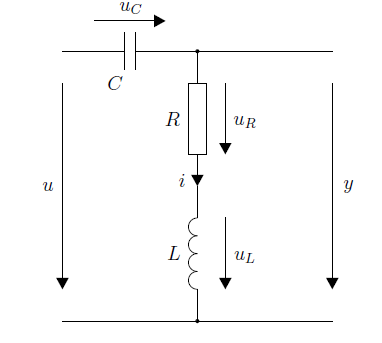
\includegraphics[width=6cm]{./images/diffgleichung.png}
		\end{center}
	\columnbreak
\begin{center}
	\begin{tabular}{ll}
		$i(t) = C \cdot \dot{u}_{C}(t)$ & Kapazität  \\
		$u_{L}(t) = L \cdot \dot{i}(t)$ & Induktivität \\
		$u_{R}(t) = R \cdot i(t)$ & Widerstand \\
		$u(t) = u_{C}(t) + u_{R}(t) + u_{L}(t)$ & Maschengleichung, links \\
		$y(t) = u_{R}(t) + u_{L}(t)$ & Maschengleichung, rechts \\
	\end{tabular}
\end{center}
\end{multicols}

\begin{multicols}{2}
{	$I(s) = C  \cdot  [s  \cdot  U_{C}(s) - u_{C}(0)]$ \\
	$U_{L}(s) = L  \cdot  [s  \cdot  I(s) - i(0)]$ \\
	$U_{R}(s) = R  \cdot  I(s)$ \\
	$U(s) = U_{C}(s) + U_{R}(s) + U_{L}(s)$ \\
	$Y (s) = U_{R}(s) + U_{L}(s)$ \\}

	\columnbreak
\begin{center}

$Y(s) = \frac{s^2 LC+sRC}{s^2 LC +sRC +1}\cdot U(s) + \frac{[sLC + RC] \cdot u_{C}(0) + L \cdot i(0)}{s^2 LC +sRC +1}$
\end{center}
\end{multicols}

Auch hier beinhaltet das Gleichungssystem 5 Gleichungen und 6 Signale. Das Eliminieren der 4 internen Signale $(U_{C}, U_{R}, U_{L}, I)$ fällt hier leichter. Offensichtlich sind hier weniger Anfangsbedingungen nötig als wenn nur eine Gleichung in den Bildbereich transformiert wird.


\subsection{Partialbruchzerlegung (PBZ)}
\subsubsection{Allgemeines Vorgehen}			\[f(x)=\frac{x^2+20x+149}{x^3+4x^2-11x-30} \Rightarrow \; \Rightarrow x^{3}+4x^{2}-11x-30=(x+2)(x^{2}+2x-15)=(8x+2)(x+5)(x-3)\]
			Ansatz:
			\[f(x)=\frac{x^2+20x+149}{x^3+4x^2-11x-30}=\frac{A}{x-3} + \frac{B}{x+2} + \frac{C}{x+5}=
			\frac{A(x+2)(x+5)+B(x-3)(x+5)+C(x-3)(x+2)}{(x-3)(x+2)(x+5)}\]
			Gleichungssystem \textbf{(Z"ahler gleichsetzen)} aufstellen mit beliebigen $x_i$-Werten (am Besten Polstellen oder 0,1,-1 w"ahlen):
			\[\begin{array}{l}x_1=3:\;-9+60+149=A\cdot5\cdot8\;\;\;\Rightarrow A=5\\
			x_2=-2:\;-4-40+149=B(-5)\cdot3\; \Rightarrow B=-7\\
			x_3=-5:\;-25-100+149=C(-8)(-3) \Rightarrow C=1 \end{array} \Rightarrow f(x)=\frac{5}{x-3}+\frac{7}{x+2} + \frac{1}{x+5}\]
%			weitere Ans"atze f"ur andere Typen von Termen: (Mehrere Werte f"ur $x$ verwenden, auch wenn kein Koeffizient 0 wird.)
%			\[f(x)=\frac{5x^2-37x+54}{x^3-6x^2+9x}=\frac{A}{x}+\frac{B}{x-3}+\frac{C}{(x-3)^2}=\frac{A(x-3)^2+Bx(x-3)+Cx}{x(x-3)^2}\]
%			\[f(x)=\frac{1,5x}{x^3-6x^2+12x-8}=\frac{A}{x-2}+\frac{B}{(x-2)^2}+\frac{C}{(x-2)^3}=\frac{A(x-2)^2+B(x-2)+C}{(x-2)^3}\]
%			\[f(x)=\frac{x^2-1}{x^3+2x^2-2x-12}=\frac{A}{x-2}+\frac{Bx+C}{x^2+4x+6}=\frac{A(x^2+4x+6)+(Bx+C)(x-2)}{(x-2)(x^2+4x+6)}\]
\subsubsection{Bedingungen}
\begin{itemize}
\item Bedingung 1: In der gezeigten Form kann die PBZ nur durchgeführt werden,
wenn die Pole paarweise verschieden sind: $p_{i} \neq p_{j}$ falls i $\neq$ j.
\item Bedingung 2: In der gezeigten Form kann die PBZ nur durchgeführt werden, wenn m < n. Die Schrittantwort des Systems ist dann stetig.
\item Bei komplex-konjugierten Polen $p_{j} = p^{\ast}_{i}$ ergeben sich komplex-konjugierte Faktoren
$c_{j} = c^{\ast}_{i}$ . Werden die entsprechenden zwei Terme addiert, ergeben sich
für die Summe reelle Koeffizienten (PT2-Glied):
\end{itemize}
\subsubsection{Standardfall}

\[ G(s) =\frac{c_{1}}{s+3} + \frac{c_{2}}{s+5} + \frac{c_{3}}{s+7} \quad \text{ mit } \quad {c_{i}= \frac{Z(s)}{\frac{dN(s)}{ds}}\mathop{\Bigg|_{s=p_{i}}}}\]

Beispiel: \[\frac{22s +35}{(s+1)(s+2)}=\frac{c_{1}}{s+1}+\frac{c_{2}}{s+2}=\frac{\frac{22s+35}{2s+3}\mathop{\Big|_{s=-1}}}{s+1}+\frac{\frac{22s+35}{2s+3}\mathop{\Big|_{s=-2}}}{s+2}=\frac{13}{s+1}+\frac{9}{s+2}\]
kann durch PBZ in drei parallel geschaltete PT1-Glieder umgeformt werden. Die
Faktorisierung ist dabei nur beim Nenner nötig.

\subsubsection{Nichtminimale Übertragungsfunktion}
\[G(s) =\frac{8s^{2} + 80s + 200}{s^3 + 15s^2 + 71s + 105}= \frac{4}{s+3} + \frac{0}{s+5} + \frac{4}{s+7}\]
Die in (27) gegebene UTF scheint zwar ein System dritter Ordnung zu sein; die beiden
folgenden Darstellungen zeigen aber, dass das I/O-Verhalten nur einem System
zweiter Ordnung entspricht. In der faktorisierten Form äussert sich dies durch
eine Pol-/Nullstellenkürzung; in der PBZ ist der entsprechende Koeffizient $c_{2}$ = 0.
Die UTF in ist nicht minimal; eine vollständig gekürzte UTF dagegen heisst
minimal.

\subsubsection{Übertragungsfunktion mit komplexen Polen}
\[G(s) =\frac{8s^{2} + 70s + 134}{s^3 + 15s^2 + 81s + 175}= \frac{8s^2+70s+134}{(s+7)(s+4+3j)(s+4-3j)}=\frac{2}{s+7}+\underbrace{\frac{3+2j}{s+4-3j}+\frac{3-2j}{s+4+3j}}\]
\textcolor{white}{x} \hspace{14.5cm} $\frac{6s+12}{s'2+8s+25}$\\

Grundsätzlich kann G(s) wieder als Parallelschaltung dreier PT1-Glieder aufgefasst
werden. Glieder mit komplexen Werte für Verstärkung und Zeitkonstante werden
üblicherweise aber zu Teilsystemen zweiter Ordnung zusammengefasst.

\subsubsection{Fall m $>$ n}
UTF mit m $>$ n haben bei hohen Frequenzen differentierendes Verhalten, mit m = n
haben sie bei hohen Frequenzen Proportionalverhalten. Um solche UTF in eine
parallele Form zu bringen, kann mit einer Polynomdivision gearbeitet werden. Die Polynomdivision wird abgebrochen, bevor negative s-Potenzen entstehen. Terme mit nicht-negativen s-Potenzen haben proportionales
bzw. differentierendes Übertragungsverhalten; bei höheren s-Potenzen träte auch
mehrfache Differentiation auf. Wenn ein übrig bleibt, so kann dieser mit PBZ weiter zerlegt werden.

\subsection{Darstellung und Eigenschaften von UTF}

\begin{eqnarray}
G(s)=\frac{Z(s)}{N(s)}=\frac{b_{m}s^m + b_{m-1}s^{m-1}+ ... + b_{1}s+b_{0}}{s^{n}+a_{n-1}s^{n-1} + ... + a_{2}s^{2}+a_{1}s + a_{0}} \\ = K\cdot \frac{(s-z_{1})(s-z_{2})...(s-z_{m})}{(s-p_{1})(s-p_{2})...(s-p_{n})} \\ = \frac{c_{1}}{s-p_{1}} + \frac{c_{2}}{s-p_{2}} + ...  + \frac{c_{n}}{s-p_{n}}
\end{eqnarray}

\begin{equation}
K=b_{m}
\end{equation}
\subsubsection{Übertragungsfunktion UTF}
\hspace{2.3cm}G(s)\\
$Y(s) = \underbrace{\frac{\overbrace{s^2 LC+sRC}}{s^2 LC +sRC +1}\cdot U(s)} + \underbrace{\frac{[sLC + RC] \cdot u_{C}(0) + L \cdot i(0)}{s^2 LC +sRC +1}}$ \newline
\textcolor{white}{x} \hspace{2.4cm} $Y_{E}(s)$ \hspace{3.8cm} $Y_{F}(s)$ \\
Das Ausgangssignal Y (s) setzt sich aus den beiden Termen $Y_{E}(s) und Y_{F}(s)$ zusammen.Der erzwungene Anteil $Y_{E}(s)$ ist durch das Eingangssignal U(s) bestimmt, aber unabhängig von den Anfangsbedingungen des Netzwerks.
Beim freien Anteil $Y_{F}(s)$ ist es umgekehrt; dieser hängt nur von den Anfangsbedingungen,
nicht aber vom Eingangssignal ab. Die freie Antwort zeigt also, wie
das System sich verhält, wenn man es ‘sich selbst überlässt’
$\text{für} u_{C}(0) \neq 0 \text{ und } \diagup \text{ oder } i_{L}(0) \neq 0$
\begin{itemize}
	\item $ y_{F}(t) die Form y_{F,1} \cdot e^{\lambda_{1}t} + y_{F,2} \cdot e^{\lambda_{1}t} \text{ haben muss, wobei}$
	\item $ \lambda_{1,2}= \frac{-RC \pm \sqrt{(RC)^2 - 4 \cdot LC} }{2 \cdot LC}$ die Wurzeln des charakteristischen Polynoms sind,
	\item und die Werte $y_{F,1} \text{ und } y_{F,2}$ sich aus den Anfangsbedingungen ergeben.
\end{itemize}
Offensichtlich ist die freie Antwort $Y_{F}$ dann von Bedeutung, wenn man an ganz konkreten
Signalwerten interessiert ist, sonst wird der Fokus jedoch auf $Y_{E}$ gelegt. \\
Die erzwungene Antwort $Y_{E}(s) = G(s) \cdot U(s)$ kann als Produkt geschrieben werden, wobei G(s) der Übertragungs-funktion entspricht.

\subsubsection{minimalphasig}
wenn keine Nullstelle $z_i$ in der rechten Halbebene liegt und die Totzeit $T_t = 0$ ist.
Motivation für den Ausdruck ‘minimalphasig’: bei stabilen Systemen hat ein
minimalphasiges System bei gegebenem Amplitudengang den minimal möglichen
Phasenabfall im Phasengang.
\subsubsection{Reaslisierbarkeit}
mit m = 3 und n = 2 illustriert, dass UTF mit $m > n$ differentierendes Verhalten
aufweisen, solche mit m = n proportionales Verhalten; der ‘Rest’ mit $m < n$ ist
ein Tiefpass. Systeme mit m $\leq$ n werden als realisierbar bezeichnet. Motiviert wird
diese Bezeichnung dadurch, weil für ein Schrittsignal am Eingang ein P-Glied ideal
funktionieren kann, ein D-Glied aber nicht. Praktisch bedeutet das, dass bei einem Regler nicht mehr Nullstellen als Pole
eingebaut werden dürfen.
\subsubsection{Minimalität}

Eine UTF mit Nennergrad n ist minimal, wenn keine Pol-Nullstellenkürzung
möglich ist. Um die UTF zu realisieren, sind dann mindestens n Integratoren nötig.\\
keine Pol-/Nullstellenkürzung möglich ist. Zu beachten ist, dass Kürzungen in
der rechten Halbebene normalerweise nicht erlaubt sind, da durch sie Instabilitäten
in einem System unsichtbar werden.

\subsubsection{Stabilität}
\begin{itemize}
\item  ist asymptotisch stabil, wenn
alle Pole pi in der linken Halbebene liegen (ohne Imaginärachse).
\item  ist grenzstabil, wenn
\begin{itemize}
\item kein Pol in der rechten Halbebene liegt und
\item mindestens ein Pol auf der Imaginärachse liegt und
\item alle Pole auf der Imaginärachse einfache Pole sind.
\end{itemize}
\item  ist instabil, wenn
sie weder asymptotisch stabil noch grenzstabil ist.
\item  ist stabil, wenn
sie asymptotisch stabil ist.
\end{itemize}


\subsubsection{Stabilitätskriterien, Routh-Kriterium}

Eine notwendige Stabilitätsbedingung für das charakteristische Polynom besteht darin, dass alle Koeffizienten positiv sind. (Vorzeichenbedingung)
\begin{equation}
\boxed{N(s) = a_{n}s^n + a_{n-1}s^{n-1} + . . . + a_2s^2 + a_1s + a_0 mit an > 0}
\end{equation}
Sind bei einem Polynom alle Koeffizienten negativ (inklusive $a_n$), ist die obige
notwendige Bedingung sinngemäss ebenfalls erfüllt.



Da dies keine hinreichende Bedingung ist muss bei bestehen des Kriteriums mit positiven Koeffizienten auch das Routh Kriterium erfüllt sein.
\begin{itemize}
	\item Die Tabelle hat n + 1 Zeilen mit den Indizes n . . . 0.
	\item In die beiden oberen Zeilen werden die Koeffizienten ai gefüllt. Je nach Systemordnung
	kommt dabei der letzte Koeffizient a0 in die erste oder zweite Zeile.
	
	\item {Jede der weiteren Zeilen der Tabelle ergibt sich durch algebraisches Rechnen
	mit den Einträgen der zwei darüber liegenden Zeilen. Das Muster der Berechnung
	wiederholt sich dabei in jeder Zeile.\\
	\begin{tabularx}{\textwidth}{XXX}
	$b_1=\frac{a_{n-1}a_{n-2}-a_{n}a_{n-3}}{a_{n-1}}$
	& $b_2=\frac{a_{n-1}a_{n-4}-a_{n}a_{n-5}}{a_{n-1}}$
	& $b_3=\ldots$ \\
	$c_1=\frac{b_{1}a_{n-3}-a_{n-1}b_{2}}{b_{1}}$
	& $c_1=\frac{b_{1}a_{n-5}-a_{n-1}b_{3}}{b_{1}}$
	& $c_3=\ldots$ \\
	$d_1=\frac{c_{1}b_{2}-b_{1}c_{2}}{c_{1}}$
	& $d_2=\ldots$ & \\
	\end{tabularx}}
	\item Durch dieses Vorgehen ergibt sich eine Dreiecksstruktur; die Tabelle endet mit
	genau einem Eintrag in Zeile 0.
	\item Die Auswertung der Tabelle besteht durch Inspektion der (grau unterlegten)
	ersten Kolonne: dass alle Koeffizienten dieser Kolonne positiv sind, ist eine
	notwendige und hinreichende Bedingung für (asymptotische) Stabilität.
\end{itemize}
\begin{table}
	\begin{tabularx}{0.6\textwidth}{|X||X|X|X|X|X|X|}
	\hline
		n & \cellcolor{hellgrau}$a_n$ & $a_{n-2}$ & $a_{n-4}$ & $\ddots\vdots$ & $a_{2}$  & $a_{0}$ \\ \hline
		n-1 & \cellcolor{hellgrau} $a_{n-1}$ & $a_{n-3}$ & $a_{n-5}$ & $\vdots\ddots$ & $a_{1}$  & 0 \\ \hline\hline
		n-2 & \cellcolor{hellgrau} $b_{1}$ & $b_{2}$ & $b_{3}$ & $\cdots$ & $b_{n/2}$  & 0 \\ \hline
		n-3 & \cellcolor{hellgrau} $c_{1}$ & $c_{2}$ & $\cdots$ & $c_{(n-2)/2}$ & 0 & 0 \\ \hline
		n-4 & \cellcolor{hellgrau} $d_{1}$ & $\ddots$ & $\ddots$ & $\ddots$ & 0 & 0 \\ \hline
		$\vdots$ & \cellcolor{hellgrau} $\vdots$ &  $\ddots$ & $\ddots$ & $\ddots$ & 0 & 0 \\ \hline
		0 & \cellcolor{hellgrau} $x_1$ & 0 & 0 & 0 & 0 & 0 \\ \hline
	\end{tabularx}
\caption{Routh-Algorithmus}
\end{table}

\subsubsection{Dominaten Pole und Nullstellen}

\begin{equation}
\boxed{Y(s)=\frac{K}{s(sT+1)}=K\mathop{\Big[}\frac{1}{s}-\frac{1}{s+\frac{1}{T}}\mathop{\Big]} \laplace K\mathop{\Big[}1-e^{\frac{-1}{T}}\mathop{\Big]}=y(t)}
\end{equation}
		\begin{center}
			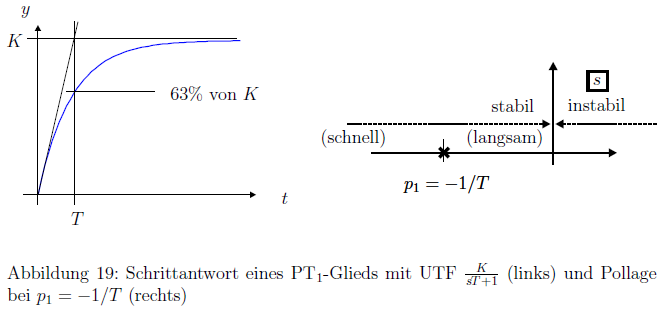
\includegraphics[width=15cm]{./images/PoleNullstellen.png}
		\end{center}
um eine schnelle Reaktion der Strecke
zu erreichen, sind grosse Werte am Reglerausgang nötig. Das bedeutet, dass man
T nicht beliebig klein machen kann, bzw. den Pol $p_1$ nicht beliebig weit nach links
legen darf.\\

Das $PT_2$-Glied hat eine UTF mit den drei Parametern K, $\xi$ und T (bzw. $\omega$ n = 1/T ).
\begin{equation}
\boxed{\frac{Y(s)}{R(s)}=G(s)=\frac{K}{s^2T^2+2\xi Ts+1}=\frac{K\omega^{2}_{n}}{s^2 + 2\xi \omega_{n}s+\omega^{2}_{n}}}
\end{equation}
\begin{itemize}
\item Modifikation
von K verändert die Höhe der Schrittantwort durch Strecken/Stauchen in
vertikaler Richtung. (Signalwerte)
\item Modifikation von T (bzw. $\omega n$) verändert
die Schrittantwort durch Strecken/Stauchen in horizontaler Richtung. (Zeit)
\item Abhängig von $\xi$ ergeben sich folgende Fälle:
\begin{itemize}
\item Fall mit $\xi$ < 0
Da T als positiv angenommen wird, ergibt sich für $\xi$ < 0 gemäss Vorzeichenbedingung
ein instabiles System.
\item Fall mit $\xi$ = 0
Dies ergibt einen harmonischen Oszillator; die Pole liegen bei $\pm j\omega_{n}$.
NB: die Periode der Oszillation entspricht nicht der Zeitkonstanten T.
\item Fall mit $ 0 < \xi < 1$
Hier resultiert ebenfalls eine Schwingung mit einer Periode; allerdings ist
die Schwingung gedämpft. Dieser Fall wird unten genauer betrachtet.
\item Fall mit $1 \leq \xi$
Dies entspricht dem aperiodischen Fall. Für (35) ist eine Faktorisierung
mit reellen Werten T1,2 möglich:
Für $\xi$ = 1 ist T1 = T2 = T; das $PT_2$-Glied entspricht der Serieschaltung
zweier identischer PT1-Glieder.
Für $\xi$ > 1 ist $T_1 > T > T_2$; das $PT_2$-Glied entspricht der Serieschaltung
zweier unterschiedlicher PT1-Glieder.
Für $\xi \gg 0$ wird mit $T_1 \gg T_2$ die Zeitkonstante T1 dominant. Das $PT_2$-
Glied verhält sich ähnlich wie ein $PT_1$-Glied
\end{itemize}
\end{itemize}

\[p_{1,2}=\frac{-2\xi\omega_n \pm \sqrt{4\xi^2 \omega^2_n - 4\omega^2_n}}{2}=\underbrace{-\xi\omega_n} \pm \underbrace{\sqrt{\xi^2-1}\cdot \omega_n}\]
\textcolor{white}{x} \hspace{10.5cm} $\sigma$ 
\hspace{1.5cm} $j\omega$
\begin{eqnarray}
\sigma=-\xi\omega_n \quad und \quad \omega=\sqrt{1-\xi^2}\cdot \omega_n  \quad bzw. \\ \omega_n=\sqrt{\omega^2 + \sigma^2}  \quad und  \quad \xi = -\frac{\sigma}{\omega_n}=-\frac{\sigma}{\sqrt{\omega^2 + \sigma^2}}\label{xiOmega}
\end{eqnarray}

Die Schrittantwort eines $PT_2$-Glieds mit $|\xi| < 1$ ergibt
\begin{equation}
\boxed{Y(s)=\frac{K\omega^2_n}{s(s^2+2\xi\omega_n s +\omega^2_n)}\laplace K\mathop{\Big[}1-e^{\sigma t}\mathop{\Big[}cos(\omega t)-\frac{\sigma}{\omega}sin(\omega t)\mathop{\Big]}\mathop{\Big]}=y(t)}
\end{equation}
\begin{multicols}{2}
\begin{itemize}
\item K ergibt sich durch $y_\infty$.
\item $\omega$ ergibt sich durch die Periode $T_\omega$ = 2$\pi$/$\omega$ [= $2T_m$].
\item $\sigma$ ergibt sich durch die Überschwingweite ym aus der Formel $y_m/y_\infty = e^{
\frac{\sigma}{\omega}\pi}$.
\item $\omega$n und $\xi$ ergeben sich gemäss (\ref{xiOmega}) aus $\omega$ und $\sigma$.
\end{itemize}
	\columnbreak
\begin{center}
	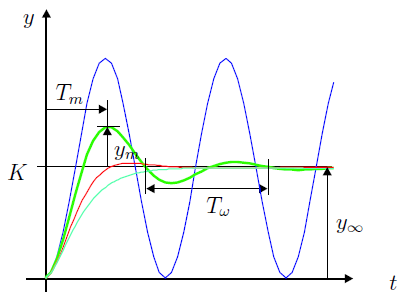
\includegraphics[width=6cm]{./images/pt2.png}
\end{center}
\end{multicols}

\subsubsection{Minimalphasigkeit}
Gegenüber den Polen werden die Nullstellen oft etwas vernachlässigt. Trotzdem
gibt es auch Fälle, in denen durch ungünstige Lage von Nullstellen regelungstechnische
Probleme erschwert werden. Beispiele sind Nullstellen in der rechten Halbebene,
durch die ein System nichtminimalphasig wird.
\subsubsection{Totzeit, Padé-Approximation}
\begin{equation}
\boxed{e^{-sT_t}=e^x\mathop\mid\limits{_{x=-sT_t}} \quad mit \quad e^x\approx 1 \approx \frac{2+x}{2-x} \approx \frac{12+6x+x^2}{12-6x+x^2} \approx \ldots}
\end{equation}
\begin{itemize}
\item  Sie ist stabil, unabhängig von der Ordnung.
\item  Die Nullstellen der Approximation entsprechen — an der Imaginärachse der
komplexen Ebene gespiegelt — den Polen. Beim Ersetzen eines Totzeitglieds
bleibt damit die Allpasseigenschaft erhalten mit $|G(j\omega)| = 1$. Weiter bleibt
auch die Nichtminimalphasigkeit erhalten.
\item  Ihr Phasengang konvergiert mit zunehmender Ordnung gegen denjenigen des
Totzeitglieds $e^{-sT_t} : \angle e^{-j\omega T_t} = -\omega T_t$.
\end{itemize}

\subsection{Blockdiagramm Algebra}
\begin{center}
	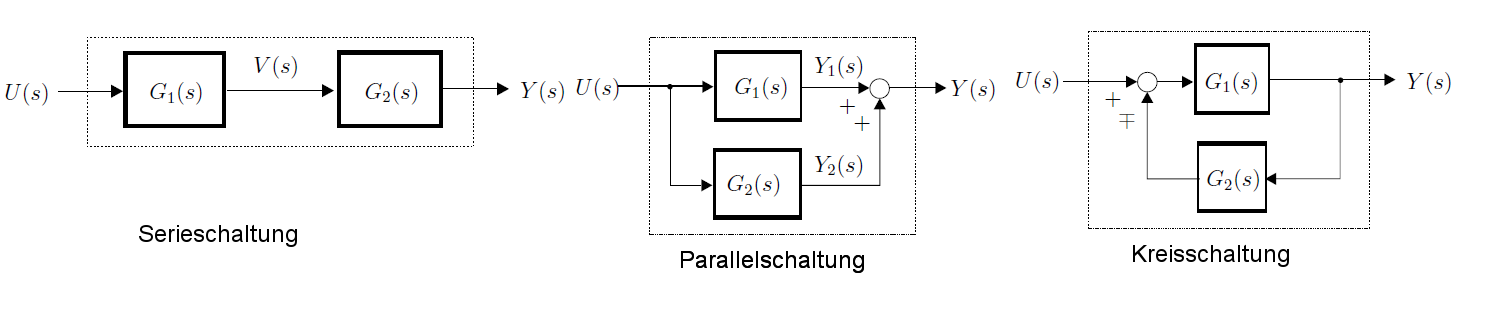
\includegraphics[width=16cm]{./images/blockdiagrammAlgebra.png}
\end{center}
\begin{itemize}
\item Zwei Blöcke hintereinander 
\begin{itemize}
	\item $U(s) \longrightarrow G_1(s)\longrightarrow G_2(s) \longrightarrow Y(s) \quad ergibt  \quad G(s)=G_1(s)\cdot G_2(s)$
	\item $Y(s) = G(s)=G_1(s)\cdot G_2(s) \cdot U(s)$
\end{itemize}
\item Zwei Blöcke Parallel
\begin{itemize}
	\item $G(s) = G_1(s) + G_2(s)$
	\item $Y_1(s) = G_1(s)\cdot U(s), Y_2(s) = G_2(s)\cdot U(s) \quad und \quad  Y(s) = Y_1(s)+ Y_2(s)$
	\item ergibt: $Y(s)= (G_s(s)+G_2(s))\cdot U(s)$
\end{itemize}

\item Kreisschaltung
\begin{itemize}
	\item $G(s) = \frac{G_1(s)}{1\pm G_1(s)\cdot G_2(s)}$
	\item $Y(s) = \frac{G_1(s)}{1\pm G_1(s)\cdot G_2(s)} \cdot U(s)$
\end{itemize}
\end{itemize}
\begin{center}
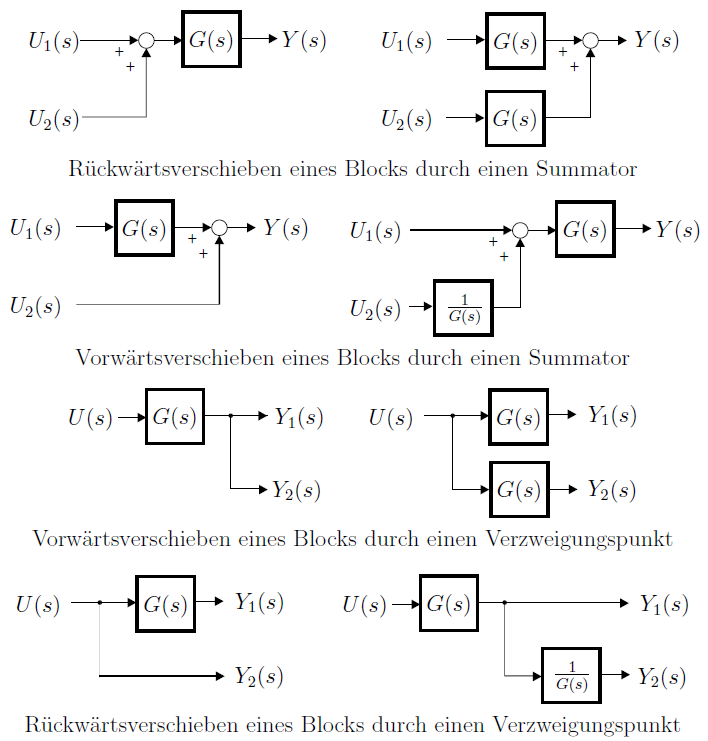
\includegraphics[width=8cm]{./images/blockdiagrammAlgebra2.png}
\end{center}


\subsection{Bodediagramm und Nyquistdiagramm}
\subsubsection{Einleitung}
\begin{itemize}
	\item Ist der offene Regelkreis stabil, muss man aufpassen, dass durch das Schliessen
	des Regelkreises (bzw. der Kreisschaltung) der geschlossene Regelkreis nicht instabil
	wird.
	\item Ist dagegen der offene Regelkreis instabil, dann kann untersucht werden, unter
	welchen Bedingungen der geschlossenen Regelkreis stabil werden kann.
	\item Das
	spezielle (oder vereinfachte) Nyquistkriterium kann nur dann angewendet werden,
	wenn der offene Regelkreis ein System mit Ausgleich ist;
	\item Beim allgemeinen Nyquistkriterium
	kann der offene Regelkreis ein beliebiges LZI-System sein, insbesondere also auch
	ein instabiles.
\end{itemize}
\subsubsection{Nyquistkriterium}
		Der geschlossene Regelkreis ist genau dann stabil, wenn beim Durchlauf der
		Ortskurve in Richtung zunehmender Frequenz der kritische Punkt -1 \glqq zur
		Linken\grqq\ liegt.

\subsubsection{Anwendung des Allgemeinen Nyquistkriteriums}
\begin{enumerate}
\item Die Anzahl N der Pole von G0, die in der rechten Halbebene oder auf der
imaginären Achse liegen, muss bestimmt werden. $(0 \leq N \leq n)$
\item Beide Äste der Ortskurve von $G_0(j\omega)$ müssen gezeichnet werden.
\item Umschlingt die Ortskurve den kritischen Punkt -1 genau N mal positiv (im
Gegenuhrzeigersinn), dann ist der geschlossene Regelkreis 
$\frac{Y(s)}{R(s)} = \frac{G_0}{1+G_0}$ asymptotisch stabil.
\end{enumerate}
Beispiel: $G_0(S)= K\cdot\frac{1}{s}\frac{1}{(s+1)^2}$
Wegen des Integrators ist N = 1. Dies bedeutet, dass der kritische Punkt
einmal im Gegenuhrzeigersinn umschlungen werden muss.\\
\begin{tabularx}{\textwidth}{XXX}
$K > 2$ & $Anzahl Umschlingungen: -1$ & Regelkreis instabil \\
$2 > K > 0$ & Anzahl Umschlingungen: 1 & Regelkreis (asymptotisch) stabil\\
$0 >K$ & Anzahl Umschlingungen: 0 & rightarrow Regelkreis instabil\\
\end{tabularx}
\subsection{Modellredution}

Tendenziell versucht man bei einer Modellreduktion, die tieffrequenten Eigenschaften
beizubehalten und dafür Ungenauigkeiten in den höheren Frequenzbereichen in
Kauf zu nehmen. Beim Modell $G_M$ wird also am ehesten $T_2$ als vernachlässigbar
klein betrachtet, womit sich folgendes reduzierte Modell $\overline{G}_M$ ergibt
\[G_M(s)=K\cdot\frac{1}{1+T_1s}\cdot\frac{1}{1+2\xi T_2 s +T^2_2 s^2} \quad wird zu \quad \overline{G}_M(s)=K\cdot\frac{1}{1+T_1s}\]
\section{Reglerentwurf \buchSeite{80}}
\subsection{Stationärer Zustand und Fehler \buchSeite{80}}
\[ G_0(s) = K_0 \cdot \frac{1}{s^{\nu}} \cdot \underbrace{\text{"'Rest"'}}_\textrm{DC-Verstärkung = 1} \]
Die UTF des offenen Regelkreises setzt sich dabei aus derjenigen von Strecke
und Regler zusammen: $G_0(s) = G_S(s)\cdot G_R(s)$. Es wird davon ausgegangen, dass $G_0$
vollständig gekürzt ist und vom Typ $\nu$ ist d.h. $\nu$ offene Integratoren hat, bzw. $\nu$ Pole
bei Null:
\begin{table}[h!]
	\begin{tabularx}{\textwidth}{|l||X|X|X|}
	\hline
		& $r(t)=A\cdot\varepsilon(t) \quad $ Sprung & $r(t)=A\cdot t \quad$ Rampe & $r(t)=A\cdot \frac{t^2}{2} \quad$ Parabel \\ 
		\hline\hline
		$\nu =0 \ (Typ \ 0) \quad P-Verhalten$ & $e_\infty=\frac{A}{1+K_0}$ & $e_\infty=\infty$ & $e_\infty=\infty$ \\ \hline
		$\nu =1 \ (Typ \ 1) \quad  I-Verhalten$ & $e_\infty=0$ & $e_\infty=\frac{A}{K_0}$ & $e_\infty=\infty$ \\ \hline
		$\nu =2 \ (Typ \ 2) \quad  I^2-Verhalten$ & $e_\infty=0$ & $e_\infty=0$ & $e_\infty=\frac{A}{K_0}$ \\ \hline
	\end{tabularx}
\end{table}
\subsection{Spezifikationen für das dynamische Verhalten \buchSeite{83}}
\begin{equation*} 
	G_f(s)=\frac{Y(s)}{R(s)}=\frac{G_0(s)}{1+G_0(s)}
\end{equation*}
\begin{equation*}
	 \text{Sensitivität } S(s)=\frac{1}{1+G_0(s)} \qquad \text{komplementäre Sensitivität } T(s)=1-S(s)=\frac{G_0(s)}{1+G_0(s)}
\end{equation*}

\begin{center}
	\textbf{Ideal:} $\qquad S(s) = 0 \quad \rightarrow \quad T(s) =1 $
\end{center}

\begin{figure}[h]
	\begin{center}
	\begin{subfigure}[b]{8cm}
		\centering
		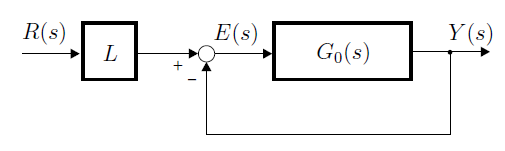
\includegraphics[width=7cm]{./images/regelkreismitL.png}
		\caption{Regelkreis mit Einheitsrückführung und Vorverstärkung L}
	\end{subfigure}\qquad
	\begin{subfigure}[b]{8cm}
		\centering
		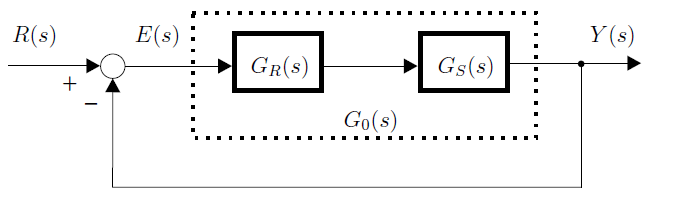
\includegraphics[width=7cm]{./images/RegelkreisEinheitsrueckfuehrung.png}
		\caption{Regelkreis mit Einheitsrückführung}
	\end{subfigure}
	\end{center}
\end{figure}
	Wird z.B. die Führungsgrösse mit einem Faktor bzw. Vorfilter L(s) vorverstärkt so ist $G_f(s)=\frac{Y(s)}{R(s)}=L(s)\cdot\frac{G_0(s)}{1+G_0(s)}$ während S(s) und T(s) erhalten bleiben.
%\begin{multicols}{2}
%		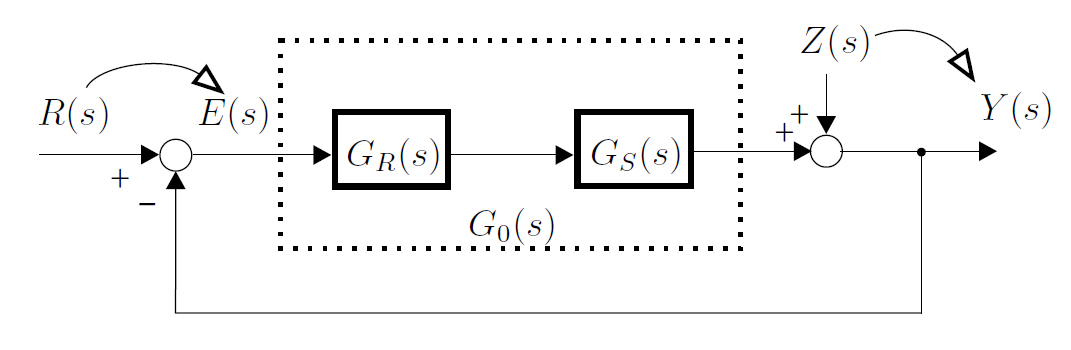
\includegraphics[width=9cm]{./images/SensitivitaetsUTF.png}
%\columnbreak
%
%Wegen $S(s) = \frac{1}{1+G_0(s)}$ ist auch der Verlauf von $S(j\omega)$ plausibel: kleine Verstärkung
%bei tiefen Frequenzen und $S(j\omega) \approx 1$ bei hohen Frequenzen. Abb. \ref{SensitivitaetRegelkreis} zeigt,
%dass $S(s) = \frac{E(s)}{R(s)}$ gilt; hochfrequente Führungssignale $r(t)$ erscheinen somit praktisch
%ungefiltert im Regelfehler $e(t)$. Ebenso wirken wegen $S(s) = \frac{Z(s)}{Y(s)}$ hochfrequente Störungen
%$z(t)$ am Streckenausgang fast ungefiltert auf die Regelgrösse $y(t)$.
%\end{multicols}

\begin{figure}[h!]
	\begin{center}
	\begin{subfigure}[b]{9cm}
	\flushleft
			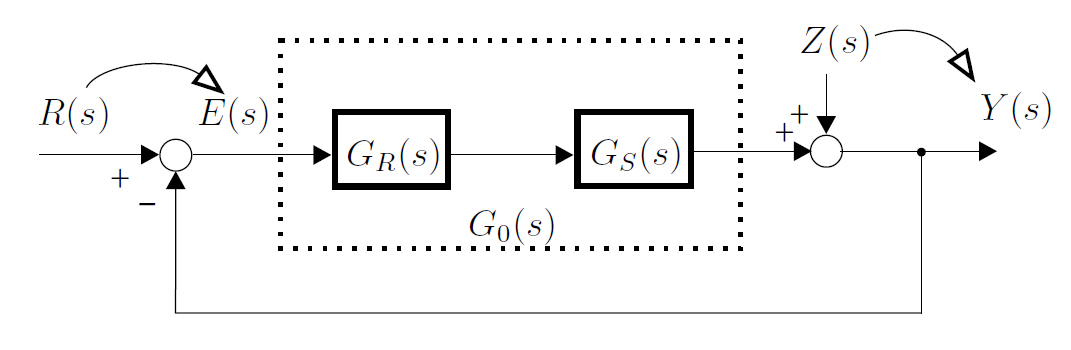
\includegraphics[width=9cm]{./images/SensitivitaetsUTF.png}
\caption{Sensitivitäts-UTF im Regelkreis, $S(s) = \frac{E(s)}{R(s)}=\frac{Z(s)}{Y(s)}$}
			\label{SensitivitaetRegelkreis}
	\end{subfigure}\qquad
	\begin{subfigure}[b]{8cm}
Wegen $S(s) = \frac{1}{1+G_0(s)}$ ist auch der Verlauf von $S(j\omega)$ plausibel: kleine Verstärkung
bei tiefen Frequenzen und $S(j\omega) \approx 1$ bei hohen Frequenzen. Abb. \ref{SensitivitaetRegelkreis} zeigt,
dass $S(s) = \frac{E(s)}{R(s)}$ gilt; hochfrequente Führungssignale $r(t)$ erscheinen somit praktisch
ungefiltert im Regelfehler $e(t)$. Ebenso wirken wegen $S(s) = \frac{Z(s)}{Y(s)}$ hochfrequente Störungen
$z(t)$ am Streckenausgang fast ungefiltert auf die Regelgrösse $y(t)$.

	\end{subfigure}
	\end{center}
\end{figure}



\subsection{Restriktionen: Bode-Integral der Sensitivität \buchSeite{87}}

Beim Erhöhen der Bandbreite $\omega_B$
besteht die Gefahr, dass in den Amplitudengängen von T und S Überhöhungen
entstehen. Werden T und S gemäss Abb. 63 als UTF T(s) = Y(s)/R(s) und
S(s) = E(s)/R(s) = Y (s)/Z(s) interpretiert, so ist auch klar, dass diese Überhöhungen
nachteilig sind. Oft wird deshalb die Spezifikationen ergänzt durch Maximalwerte für die Resonanzüberhöhung von
T und/oder S. Typische Maximalwerte sind z.B. 3-5 dB.

%\textbf{Theorem 3.1} (Bode-Integral der Sensitivität)\\
Es sei $G_0(s)$ eine gebrochen rationale Funktion mit mindestens zwei Polen mehr als Nullstellen, d.h. $n - m \geq 2$. $G_0(s)$ habe $N_p$ Pole $p_i$ in der rechten Halbebene. Dann gilt

\begin{equation}
\textrm{Bode-Integral der Sensitivität} \qquad
\int\limits_{0}^{\infty}ln|S(j\omega)|d\omega =\underbrace{\pi\cdot\sum\limits_{i=1}^{N_{p}}Re(p_i)}_\textrm{0, falls $G_0$ stabil}
\label{BodeIntegral}
\end{equation}

\begin{itemize}
	\item Ist $G_0$ stabil, dann wird der Ausdruck in (\ref{BodeIntegral}) gleich Null. Ist bei einer Frequenz
	$|S(j\omega)| < 0 \ dB$, dann muss zwingend irgendwo anders $|S(j\omega)| > 0 \ dB$ sein.
  \item Ist $G_0$ instabil, dann verschlechtert sich die Situation entsprechend.
	\item \textbf{Verkleinert man $|S(j\omega)|$ an einer Stelle, wird $|S(j\omega)|$ dafür an einer anderen
	Stelle grösser;} dies wird als ‘Wasserbetteffekt’ bezeichnet.
	Gleichung (\ref{BodeIntegral}) hat den Charakter eines Erhaltungsgesetzes.
	\item Bei den Frequenzen, bei denen
	der Aushub für ein bessere Bandbreite $\omega_B$ abgelagert wird, muss der Abstand zwischen dem Punkt -1 und der
	Ortskurve, d.h. $|1 + G_0|$, im Intervall $1 > |1 + G_0| \geq (1 + \varepsilon)-1$ liegen.
\end{itemize}

In der Praxis kann der Aushub also nicht einfach in einem beliebig hohen bzw.
breiten Frequenzband ‘entsorgt’ werden, sondern man muss Gleichung (\ref{BodeIntegral}) etwas
einschränken:
\begin{equation}
\int\limits_{0}^{\omega_M}ln|S(j\omega)|d\omega =\pi\cdot\sum\limits_{i=1}^{N_{p}}Re(p_i) \qquad \text{mit} \quad \omega_M \approx 10 \cdot \omega_B
\end{equation}
\section{Reglerentwurf mit Wurzelortskurven (WOK) \buchSeite{93}}
Wurzelortskurven beschreiben die Pole linearer Systeme in Abhängigkeit von freien
Parametern.
\begin{itemize}
	\item Bei einer
	infinitesimal kleinen Änderung eines Parameters ändern die Pole auch nur infinitesimal.
	\item Wenn die n Pole eines Systems nter Ordnung für alle Parameterwerte aufgezeichnet
	werden, erscheint die Gesamtheit der Pole deshalb als n Kurven (Äste).
	\item Diese n Äste entsprechen den geometrischen Orten der Wurzeln in der komplexen
	Ebene
	\item Mithilfe der WOK kann z.B. abgeschätzt werden,
	\begin{itemize}
	\item ob es Parameterwerte gibt, die zu einem stabilen System führen,
	\item wie gross man den freien Parameter wählen/einstellen muss,
	\item welche Dämpfungen man dabei erreichen kann.
\end{itemize}
\end{itemize}


\subsection{Zeichnen der Wurzelortskurven \buchSeite{93}}
\begin{equation}
G_f(s)=\frac{KG(s)}{1+KG(s)}=\frac{K\frac{Z(s)}{N(s)}}{1+K\frac{Z(s)}{N(s)}}=\frac{KZ(s)}{\underbrace{N(s)+KZ(s)}}=\frac{Z_f(s)}{N_f(s)}
\end{equation}
\textcolor{white}{x} \hspace{9cm} charakteristisches Polynom $N_f(s)$ 

\begin{multicols}{2}
	\begin{flushleft}
		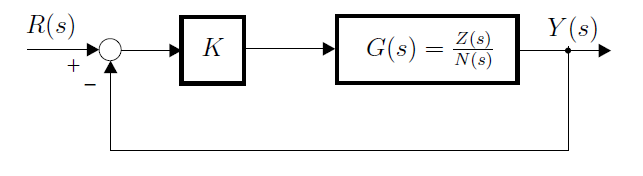
\includegraphics[width=9cm]{./images/StandardRegelkreisWOK.png}
	\end{flushleft}
\columnbreak
	\begin{flushleft}
		Beispiel: $G=\frac{1}{s-5} \quad G_f=\frac{K}{s-5+K}$ 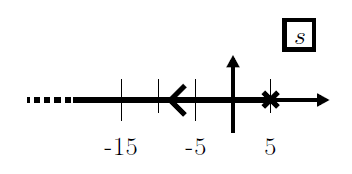
\includegraphics[width=4cm]{./images/beispielWOK.png}\\ Das charakteristische Polynom s - 5 + K zeigt eine
		Wurzel bzw. einen Pol bei s = 5 - K.
	\end{flushleft}
\end{multicols}

\subsubsection{Voraussetzungen und Vereinbarungen \buchSeite{95}}
\begin{itemize}
\item  Die UTF $G(s)=\frac{Z(s)}{N(s)}=\frac{s^m + b_{m-1}s^{m-1}+ ... + b_{1}s+b_{0}}{s^{n}+a_{n-1}s^{n-1} + ... + a_{2}s^{2}+a_{1}s + a_{0}}$
ist eine gebrochen rationale
Funktion in s mit monischen Polynomen (normierte führende Koeffizienten).
\item  In G(s) ist der Nennergrad n mindestens so gross wie der Zählergrad m; $n \geqq m$.
\item  Hat die zu untersuchende UTF eine zusätzliche Totzeit $e^{-sT_t}$ , so kann diese
z.B. mit der Padé-Approximation in die gewünschte Form gebracht werden.
\item  Hat die zu untersuchende UTF eine zusätzliche Verstärkung $k_0$, so kann diese
als Teil (d.h. als Faktor) von K betrachtet werden.
\item  Die WOK werden gezeichnet bezogen auf positive Verstärkungen K. Zu beachten
ist, dass K eine allfällig vorhandene Verstärkung k0 beinhaltet.
\end{itemize}

\subsubsection{Grundsätzliches Aussehen der WOK \buchSeite{96}}
\begin{minipage}{14cm}
	\begin{itemize}
		\item  Das charakteristische Polynom $N_f (s) = N(s)+K \cdot Z(s)$ hat für jeden K-Wert
		n Wurzeln. Visualisiert man die Wurzeln für alle positiven K-Werte, dann
		ergeben sich n kontinuierliche Linien (Äste).
		\item  Da Pole immer reell oder (paarweise) komplex-konjugiert sind, ist das Gesamtbild
		der WOK immer symmetrisch bezüglich der reellen Achse.
	\end{itemize}
\end{minipage}
\hspace{0.5cm}
\begin{minipage}{4cm}
	\textbf{Merke:} \\
		m = Anz. Nullstellen \& \\
		n = Anz. Pole von $G_0$
\end{minipage}
\begin{itemize}
		\item  Für K = 0 sind die n Wurzeln von $N_f(s)$ und N(s) identisch und entsprechen
		den n Polen von G(s).
		Für $K \rightarrow \infty$ streben m der Wurzeln von $N_f(s)$ zu den Wurzeln von Z(s). Die
		restlichen n-mWurzeln von Nf (s) streben entlang von Geraden asymptotisch
		ins ‘Unendliche’.
		Damit teilen sich die n Äste auf in zwei Arten:
		\begin{enumerate}
			\item m Äste, die von m Polen von G(s) zu den m Nullstellen von G(s) gehen
			\item n - m Äste, die von n - m Polen von G(s) ins Unendliche laufen.
		\end{enumerate}
\end{itemize}


\subsubsection{Regeln zum Zeichnen der WOK \buchSeite{96}}
\begin{enumerate}
\item \textbf{Pol-/Nullstellen-Plan:}\\
Die Pole $p_k (k = 1...n)$ von G(s) werden als x in der komplexen Ebene eingezeichnet;
dies sind die Startpunkte aller n Äste. Die Nullstellen $z_k (k = 1...m)$
werden als o eingezeichnet; dies sind die Endpunkte von m Ästen.
\item \textbf{Reelle Achse:}\\
Diejenigen Punkte der reellen Achse welche zu den WOK gehören, haben rechts
von sich auf der reellen Achse eine ungerade Anzahl von Polen und Nullstellen.
Um diese Punkte einzuzeichnen, kann man von ‘genug weit’ rechts startend
der reellen Achse entlang ‘genug weit’ nach links fahren. Dabei wechselt der
Zeichenstift bei jedem Pol und bei jeder Nullstelle den Status zwischen ‘nicht
zeichnend’ bzw. ‘zeichnend’. Der Anfangsstatus ist ‘nicht zeichnend’.
\begin{figure}[h!]
	\begin{center}
		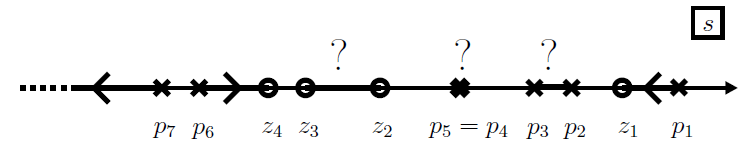
\includegraphics[width=12cm]{./images/reelleAchsePoleNullWOK.png}
	\end{center}
	\caption{Zur WOK gehörende Teile der reellen Achse}
	\label{beispielAchse}
\end{figure}

Im etwas komplexeren Beispiel von Abb.\ref{beispielAchse} entstehen 6 Striche. Einer davon
ist nur ein Punkt: beim Doppelpol $p_4 = p_5$. Einer der Striche verschwindet
gegen links im Unendlichen. Zwei Striche verbinden Pol mit Nullstelle; dies
sind gültige WOK-Äste. An den mit ? versehenen Stellen ist offensichtlich die
Situation noch unbefriedigend.


\item \textbf{Asymptoten: Schnittpunkt und Richtungen:}\\
Wenn $n > m$ gilt, dann streben n-m Äste der WOK asymptotisch gegen
Unendlich. Die n-m Asymptoten sind Geraden. Sie schneiden sich im Punkt
\begin{multicols}{2}
		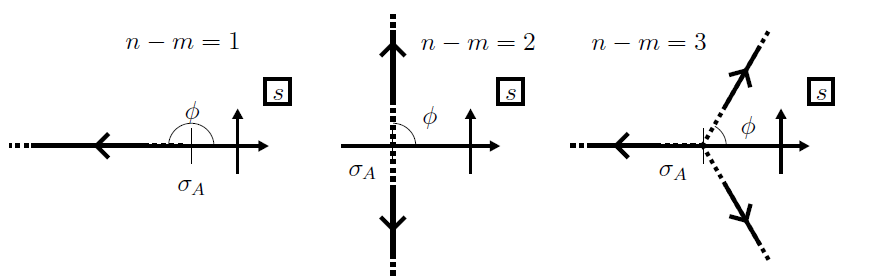
\includegraphics[width=10cm]{./images/asymptotenrichtunge.png}
Abbildung \ref{Asymptotenrichtungen}: Asymptotenrichtungen bei WOK für die Fälle n - m = 1, 2, 3 (Weitere im Anhang)
		\label{Asymptotenrichtungen}
\columnbreak
	\begin{flushright}
		\[\boxed{\sigma_A=\frac{\sum\limits_{k=1}^{n} Re(p_k)-\sum\limits_{k=1}^{m} Re(z_k)}{n-m}}\]
	\end{flushright}
\end{multicols}
Eine der Asymptoten zeigt in die Richtung $\phi = \frac{\pi}{n-m}$. Die weiteren Asymptoten
sind dann gleichmässig um den Winkel $\frac{2\pi}{n-m}$ versetzt,

\begin{multicols}{2}
\item \textbf{Verzweigungspunkte, Vereinigungspunkte:}\\
Erklärung zu den In Abb. \ref{Asymptotenrichtungen} mit ? versehenen Stellen. Treffen
zwei Äste, von Polen her kommend, aufeinander, dann verzweigt
sich die WOK. Beim Verzweigungspunkt treten die Äste (meistens) rechtwinklig
aus der reellen Achse aus. Entsprechend können auch zwei Äste im rechten
Winkel auf die reelle Achse zustreben und nach dem Vereinigungspunkt auf
dieser weiterlaufen. In Abb. \ref{KomplettWOK} ist die Skizze der WOK aus Abb. \ref{beispielAchse}
komplettiert: $\sigma_{V,1}$ ist dabei ein Vereinigungspunkt, $\sigma_{V,2}$ und $\sigma_{V,3}$ sind zwei
Verzweigungspunkte. $\sigma_{V,1}$ und $\sigma_{V,2}$ sind näherungsweise mit zwei Kreisbögen
verbunden. \\

\columnbreak
Da n-m = 3 gilt, entstehen drei Asymptoten, deren Schnittpunkt
bei $\sigma_A$ liegt.

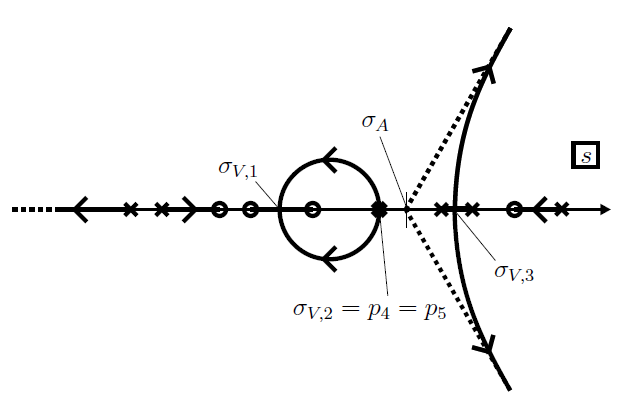
\includegraphics[width=6.5cm]{./images/KomplettWOK.png}\\
Abbildung: \ref{KomplettWOK} {Komplettierte Skizze der WOK Abb: \ref{Asymptotenrichtungen}} \label{KomplettWOK}
\end{multicols}
Für eine \textbf{einfache Skizze} genügt es meistens, die Verzweigungs- bzw. Vereinigungspunkte ‘etwa in der Mitte’ zwischen den involvierten zwei Polen bzw. Nullstellen zu plazieren.
\end{enumerate}

\subsection{Interpretation der Wurzelortskurven \buchSeite{100}}

\subsubsection{Auslegen eines P-Reglers mithilfe der WOK \buchSeite{101}}
\begin{figure}[h!]
	\begin{subfigure}[t]{8.5cm}
Beispiel: Eine Strecke \[G_s(s)=\frac{5}{s^2 + 6s +8}=\frac{5}{(s+2)(s+4)}\] soll mit einem P-Regler mit
 möglichst grosser Verstärkung $K_R$ geregelt werden, wobei alle Pole eine minimale
 Dämpfung $\xi = 0.7$ haben sollen.\\


	\end{subfigure}$\qquad$
	\begin{subfigure}[t]{10cm}
		Lösung:
		 \[G_0=K_R\cdot\underbrace{\frac{5}{(s+2)(s+4)}}_{G_s(s)}=\underbrace{K_r\cdot 5}_{K} \cdot\underbrace{\frac{1}{(s+2)(s+4)}}_{G(s)}\]
		%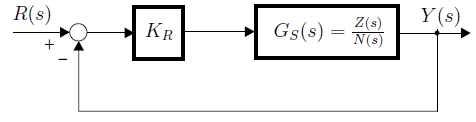
\includegraphics[width=7cm]{./images/PReglerBeispielWOK1.png}
	\end{subfigure}
\end{figure}

Zusammenfassung des Vorgehens:\\
\begin{center}
    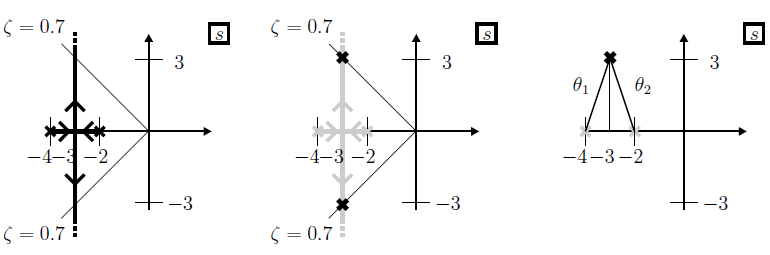
\includegraphics[width=12cm]{./images/PReglerBeispielWOK2.png}
\end{center}

\begin{multicols}{2}
    \begin{itemize}
    	\item  \textbf{Links:} Die WOK-Äste treffen sich bei -3 und laufen vertikal weiter.
    	\item  \textbf{Mitte:} Die Dämpfung nimmt mit steigendem Wert von K (bzw. $K_R$) ab; die
    	Pole kommen auf die Schnittpunkte der WOK mit den Winkelhalbierenden um eine Dämpfung von $\xi$ = 0.7 zu erreichen.
    	\item  \textbf{Rechts:} Um den Wert K (bzw. $K_R$) zu bestimmen, muss einer der platzierten	Pole betrachtet werden. Der Wert von K berechnet sich aus den Abständen $\theta_i$ dieses Pols zu den Polen von G(s) und den Abständen $\lambda_i$ dieses Pols zu den
    	Nullstellen von G(s): 
        \[
            K=\frac{\prod_{i=1}^{n} \theta_i}{\prod_{i=1}^{m}\lambda_i}=\frac{\theta_1\theta_2\cdots\theta_n}{\lambda_1\lambda_2\cdots\lambda_m} \\
        \]
        Im konkreten Beispiel hat es keine Nullstellen, womit das entsprechende Produkt
    	gleich Eins wird. 	Damit ist $K=\theta_1\theta_2$ .Mit $\theta_1=\theta_2=\sqrt{3^2+1^2}$ ergibt sich \textbf{K = 10} bzw. $K_R = K/5 = 2$.
    \end{itemize}
\end{multicols}


\subsubsection{Auslegen dynamischer Regler mithilfe der WOK \buchSeite{102}}


\subsubsection{Allgemeine Stabilitätsanalyse mithilfe der WOK \buchSeite{109}}
Der Regelkreis $K\cdot G_s(S)=K\cdot\frac{1}{S^2+\alpha s + 2}$ mit den zwei Parametern K und $\alpha$ hat das charakteristische
Polynom $N_f(s)=N(s) + K\cdot Z(s) = s2 + \alpha s + (2 + K)$. Denkt man sich jeweils einen der
Parameter als fix gegeben, kann mithilfe der WOK den Einfluss des anderen Parameters
auf die Pollage des geschlossenen Regelkreises untersucht werden:

Fall 1, $\alpha$ fix, K variabel
Dies entspricht dem bisher besprochenen Vorgehen, bei dem die Kreisverstärkung
K untersucht wird, und bei dem die Summe Nf (s) so interpretiert wird:
$N_f(s)=\underbrace{s^2+\alpha s + 2} +\underbrace{K}\cdot\underbrace{1} $\\
\textcolor{white}{x} \hspace{12.25cm} $P_N(s)=N(s) \quad Faktor  \quad P_z(s)=Z(s)$
Fall 2, $\alpha$ variabel, K fix Bei einer Untersuchung bezüglich $\alpha$ ist dagegen
$N_f(s)=\underbrace{s^2+ 2 + K} +\underbrace{\alpha}\cdot\underbrace{s} $\\
\textcolor{white}{x} \hspace{13.5cm} $P_N(s) \qquad Faktor  \quad P_z(s)$

\section{Reglerentwurf mit Bodediagramm \buchSeite{111}}

\subsection{Phasenreserve und Verstärkungsreserve \buchSeite{112}}
\begin{multicols}{2}
\begin{itemize}
\item Beim Auslegen des offenen Regelkreises sollte neben dem Nominalfall
auch den ‘worst case’ im Auge behalten werden. Auch beim letzteren sollte die
Ortskurve nicht zu knapp neben dem kritischen Punkt vorbei laufen, da dies zu
Resonanzüberhöhungen in den Sensitivitäten S(s) und T(s) führt.
\item Die rechts dargestellten Sicherheitsabstände sind bei den zwei Punkten ablesbar,
wo die Ortskurve den Einheitskreis bzw. die negative reelle Achse durchstösst.
\item Die beiden Punkte entsprechen $G_0(j\omega_D)$ und $G_0(j\omega_{\pi})$, wobei $\omega_D$ die Durchtrittsfrequenz
ist und $\omega_{\pi}$ die Phasenschnittfrequenz.
\item Der erste Punkt liefert die Phasenreserve $\Phi_{RES}$; es gilt $G_0(j\omega_D) = e^{j(-\pi+\Phi_{RES}})$. 
\item Der zweite Punkt liefert die Verstärkungsreserve$K_{RES}$; es gilt $G_0(j\omega_{\pi}) = -1/K_{RES}$. 
\item Der geschlossene Regelkreis wird grenzstabil, wenn im offenen Kreis eine zusätzliche Verstärkung $\widetilde{K} = K_{RES}$ vorhanden ist, d.h. wenn $\widetilde{G}_0 = K_{RES}G_0$.
\item Alternativ wird der geschlossene Regelkreis auch grenzstabil, wenn der offene Regelkreis eine zusätzliche Totzeit $\widetilde{T}_t = \Phi_{RES}/\omega_D$ hat,
d.h. wenn $\widetilde{G}_0 = G_0\cdot e^{-s\cdot\Phi_{RES}/\omega_D}$. Zu beachten ist, dass die beiden Typen von Reserve
miteinander gekoppelt sind.
\end{itemize}
		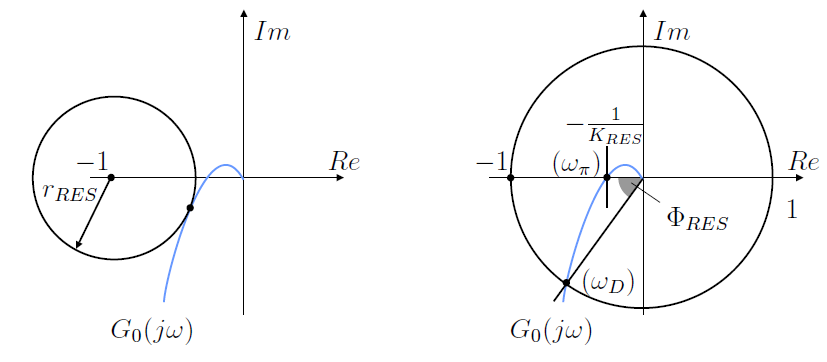
\includegraphics[width=10cm]{./images/PhasenVerstaerkungReserve.png}
\hspace*{2.5cm}Weitere Berechnungen siehe RegT1+2 Buch.
\end{multicols}
\subsection{Spezifikationen für das dynamische Verhalten (II) \buchSeite{115}}
\begin{itemize}
\item Der offene Regelkreis soll das allgemeine Nyquistkriterium
erfüllen, damit der geschlossene Regelkreis stabil wird.
\item Der offene Regelkreis soll ca. eine Phasenreserve $\Phi_{RES}$ zwischen $40^{\degree}$ und $70^{\degree}$
und eine Verstärkungsreserve $K_{RES} > 4 (\approx 12dB)$ aufweisen. Damit wird der
geschlossene Regelkreis robust gegenüber Parameterunsicherheiten und damit
bleiben auch die Überhöhungen von $|S(j\omega)|$ und $|T(j\omega)|$ limitiert.
\item Der offene Regelkreis soll eine hohe Durchtrittsfrequenz $\omega_D$ aufweisen, damit
der Regelkreis eine hohe Bandbreite $\omega_B$ hat und damit ‘schnell’ ist.
\item Die Verstärkung $|G_0(j\omega)|$ des offenen Regelkreises soll bei den tiefen Frequenzen
$\omega < \omega_D$ genug gross sein
\item Im Bereich um die Durchtrittsfrequenz $\omega_D$ sollte $|G_0(j\omega)|$ idealerweise mit
etwa 20 dB/Dekade fallen. Steilere Amplitudengänge in der Umgebung von
$\omega_D$ verkleinern die Phasenreserve $\Phi_{RES}$.\newline
Bei realen Systemen fällt $|G0(j\omega)|$ für $\omega \geqslant \omega_D$ mit mindestens 40 dB/Dekade
ab, weil sowohl Strecke wie Regler Tiefpassverhalten haben.
\end{itemize}
\subsection{Entwurfsbeispiele \buchSeite{116}}
\paragraph{Inverse Regler \buchSeite{116}} \mbox{} \\

    Dass der Regler die Inverse der Strecke enthält, ist ein gängiges Konzept. Allerdings
    kann es oft nicht vollständig umgesetzt werden. Beispielsweise darf die Strecke weder
    Pole noch Nullstellen in der rechten Halbebene haben und auch keine Totzeit enthalten

\paragraph{$\mathbf{PIDT_1}$ \buchSeite{116}}

\paragraph{Lead/Lag-Glied \buchSeite{118}}

    \begin{minipage}{6cm}
        \[ G(s) = K \cdot \dfrac{sT_1+1}{sT_2+1} \]
    \end{minipage}
    \begin{minipage}{8cm}
        Lead-Glied: $T_1 > T_2 > 0$ \newline
        Lag-Glied: $T_2 > T_1 > 0$ 
    \end{minipage}

\paragraph{Notch-Filter \buchSeite{120}}

%Schritte des Reglerentwurfs kann man sich so vorstellen
%\begin{itemize}
%\item  Der Reglerpol bei Null erzeugt bei $G_0$ die gewünschte grosse Verstärkung bei
%tiefen Frequenzen.
%\item  Die beiden Nullstellen des Regler ‘biegen’ die Kurve von $|G_0(j\omega)|$ gerade, so
%dass sie durchgehend mit 20 dB/Dekade fällt. $G_0(j\omega)$ ist jetzt konstant $-90^{\degree}$.
%Der offene Regelkreis entspräche der Idealsituation eines Integrators.
%\item  Wegen der Realisierbarkeit muss noch ein zweiter Reglerpol eingeführt werden,
%der $|G_0(j\omega)|$ bei der - relativ hohen - Frequenz $\omega$ = 20 [rad/s] wieder nach
%unten knickt und der die Phase $G_0(j\omega)$ bei höheren Frequenzen auf $-180^{\degree}$
%fallen lässt.
%\item  Mit der Verstärkung KR wird die Phasenreserve $\Phi_{RES} = 65^{\degree}$ eingestellt.
%\end{itemize}


\subsection{Bemerkungen zum Reglerentwurf mithilfe von Spezifikationen \buchSeite{122}}

Zu beachten ist, dass es einige fundamentale Einschränkungen für die Bandbreite
von Regelkreisen gibt. Folgende Abschätzungen zu
instabilen und nichtminimalphasigen Systemen:
\begin{enumerate}
\item Eine Strecke hat einen \textbf{reellen Pol p in der rechten Halbebene}. 

Will man in diesem Fall $T(j\omega) \leq 2$ halten (6 dB), muss die Bandbreite $\omega_B$
einen Mindestwert haben:
\[\omega_B > 2p\]
\item Eine Strecke hat eine \textbf{reelle Nullstelle z in der rechten 
Halbebene}.

Will man in diesem Fall eine Phasenreserve von ca. $35^{\degree}$ erreichen, muss die
Durchtrittsfrequenz $\omega_D$ limitiert werden (und damit auch die Bandbreite $\omega_B)$ \[\omega:D < z/2\]

\item Eine Strecke hat eine \textbf{Totzeit} $T_t$

Um in diesem Fall eine Phasenreserve von ca. $35^{\degree}$ zu erreichen, muss die Durchtrittsfrequenz
$\omega_D$ limitiert werden (und damit auch die Bandbreite $\omega_B$):
\[\omega_D < 1/T_t\]
\end{enumerate}
Offensichtlich gibt es also auch Situationen, in denen das Lockern von Spezifikationen
gar nichts hilft; etwa bei Kombination von Fall 1 mit Fall 2. Um einen sinnvollen
Regler entwerfen zu können, muss primär die Regelstrecke modifiziert werden.

\section{Optimierung von Reglern \buchSeite{123}}
\subsection{Reglerstrukturen \buchSeite{124}}
%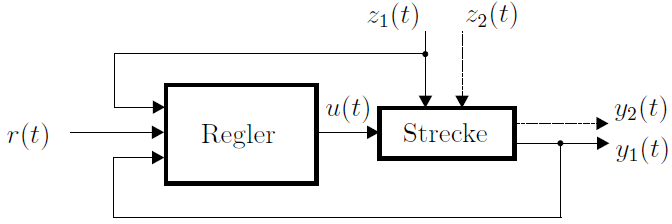
\includegraphics[width=6cm]{./images/Reglerstruktur.png}
\subsubsection{Hierarchische Regelung \buchSeite{126}}
Die verschiedenen Hierarchiestufen unterscheiden sich in einigen Punkten:
\begin{itemize}
	\item Die tiefer liegenden Regler sind ‘klassische’ Regler, die permanent gemäss einer
	Differential- oder Differenzengleichung arbeiten. In höher liegenden Schichten
	werden beispielsweise auch Zustandsautomaten und logische Grössen benutzt.
	\item Soweit man es mit ‘klassischen’ Reglern zu tun hat, arbeiten die tiefer liegenden
	Regler normalerweise mit einer höheren regelungstechnischen Bandbreite $\omega_B$.
	\item Die tiefer liegenden Regler sind meist zeitkritischer. Sie arbeiten mit höherer
	Abtastrate, allenfalls auch analog.
	\item Die oberen Stufen können die unteren Stufen auch steuern und überwachen
	bezüglich Abläufen, Fehlern, Ausfällen, Performance etc.
\end{itemize}

\subsubsection{Kaskadenregelung \buchSeite{128}}
\begin{multicols}{2}
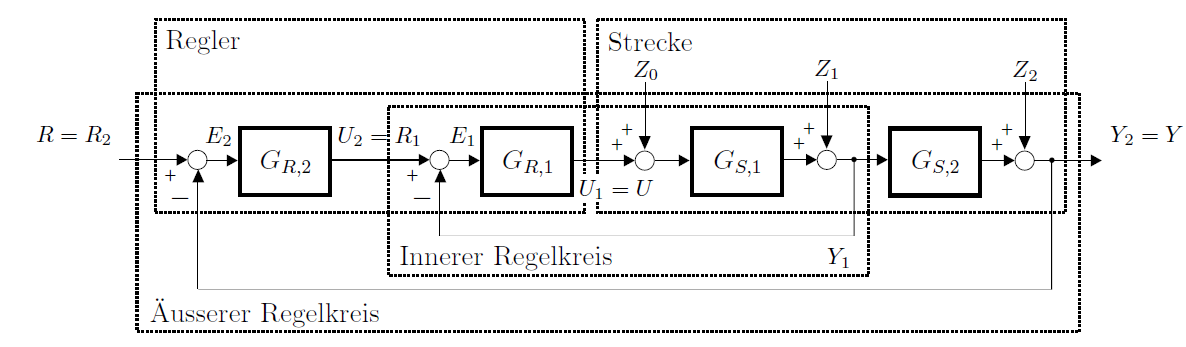
\includegraphics[width=10.5cm]{./images/KaskadenRegelung.png}
Generell gilt bei der Kaskadenregelung folgendes:
\begin{itemize}
\item Beim Reglerentwurf geht man typischerweise von innen nach aussen vor. Zuerst
wird also für die Teilstrecke GS,1 ein Regler GR,1 erstellt. Danach wird für die
fiktive Strecke $G_{S,2} \cdot \frac{G_{S,1}G_{R,1}}{1+G_{S,1}G_{R,1}}$
der Regler GR,2 ausgelegt.
\item Die inneren Regler müssen primär schnell sein; die äusseren Regler dagegen
genau. Mit dem überlagerten Regelkreis kann erzwungen werden, dass der stationäre Fehler verschwindet.
\item Wenn ein innerer Regelkreis gegenüber einem äusseren Kreis schnell ist, dann
erscheint er gegen aussen auch eher als ideales LZI-System. Z.B. kann so das
nichtlineare Verhalten von Leistungshalbleitern gegen aussen versteckt werden.
\item Tendenziell ist die Bandbreite der inneren Regelkreise also grösser zu wählen
als diejenige der äusseren Regelkreise. Dadurch wird eine zeitliche Entkopplung
erreicht; die Regler stören sich gegenseitig weniger.
Normalerweise kann mit der Kaskadenstruktur eine höhere Bandbreite und
auch eine grössere Robustheit erreicht werden gegenüber dem Fall, wenn nur
der äusserste Regelkreis geschlossen wird.
Treten bei $Z_0$ und $Z_1$ auf, reagiert bereits der Regler
$G_{R,1}$ darauf.
\item Entspricht  GS,2 einem Integrator, kann durch die
Messung von $y_1(t) = \dot{y}(t)$ vermieden werden, dass das Signal y(t) im Regler
differenziert werden muss. Dies ist ja gerade bei verrauschten Signalen nicht
zu empfehlen.
\end{itemize}
\end{multicols}

\subsubsection{Störgrössenaufschaltung \buchSeite{123}}


\subsubsection{Vorfilter, Vorsteuerung, 2DOF (Two degrees-of-freedom) \buchSeite{132}}


\subsection{Reglereinstellungen \buchSeite{123}}

%\subsubsection{Empirische Einstellregeln nach Ziegler-Nichols}
%\begin{tabularx}{0.5\textwidth}{|X||X|X|X|}
%\hline
%Regler & $K_R$ & $T_N$ & $T_V$ \\ \hline\hline
%P-Regler & $\frac{T_g}{K_s\cdot T_u}$ & - & - \\ \hline
%PI-Regler & $0.9\cdot\frac{T_g}{K_s\cdot T_u}$ & $3.33\cdot T_u$ & - \\ \hline
%PID-Regler & $1.2\cdot\frac{T_g}{K_s\cdot T_u}$ & $2\cdot T_u$ & $0.5\cdot T_u$ \\ \hline
%\end{tabularx}

\subsubsection{Optimierung mithilfe eines Gütemasses}

Zur einfacheren Beurteilung der Regelgüte wird die Information der Signale mit einer Zielfunktion auf ein
Gütemass J reduziert.
\begin{eqnarray}
J(k_1,\cdots,k_M)=\int\limits_{0}^{T_{end}}f(e(t,k_1,\cdots,k_M))dt\\
%J=\int\limits_{0}^{\infty}e(t)^2dt= \frac{1}{2\pi} \int\limits_{-\infty}^{\infty}|E(j\omega)|^2d\omega= \frac{1}{2\pi} \int\limits_{-\infty}^{\infty}E(j\omega)E^{\ast}(j\omega)d\omega\\
%J_1=\frac{b_0^2}{2a_0a_1} \qquad J_2=\frac{b_1^2a_0+b_0^2a_2}{2a_0a_1a_2} \qquad J_3=\frac{b_2^2a_0a_1+(b_1^2-2b_0b_2)a_0a_3+b_0^2a_2a_3}{2a_0a_3(a_1a_2-a_0a_3)} \qquad  \\
%\text{Bedingung: Nennerpolynom E(s) muss stabil sein}
\end{eqnarray}

\begin{itemize}
\item Die Funktion $f(e)$ wird meist so gewählt, dass $f(\overline{e}) > f(e)$ für $|\overline{e}| > |e|$.
Kandidaten sind z.B. $f(e) = |e|$ oder $f(e) = e^2$ (ISE, integral of squared
error). Grössere Werte von e werden damit "'bestraft"'; je grösser der Wert von
J ist, desto schlechter ist der Regelkreis.
\item Die Dauer $T_{end}$ des ausgewerteten Intervalls muss auf die (zu erwartenden)
Zeitkonstanten des Regelkreises abgestimmt sein. $T_{end}$ sollte mindestens so
gross sein, dass der Regelkreis bei vernünftiger Reglereinstellung als eingeschwungen gelten kann.
\item \textbf{Allgemeine Anwendung des quadratischen Gütemasses \buchSeite{139}}
\end{itemize}


\subsubsection{Vorgabe der Führungsübertragungsfunktion \buchSeite{143}}

Wie kann der Regler bestimmt werden, mit dem das gewünschte $G_f(s)$ resultiert?
Der Regler für eine Strecke $G_S(s) = Z_S(s)/N_S(s)$ und für eine geeignet gewählte
Führungs-UTF $G_f(s) = Z_f(s)/N_f(s)$ kann so berechnet werden:
\begin{equation}
\boxed{G_R(s)=\frac{Z_f(s)}{N_f(s)-Z_f(s)}\cdot\frac{N_S(s)}{Z_S(s)}}
\end{equation}
\begin{itemize}
\item  Die Strecke muss stabil sein. Andernfalls würden in der rechten Halbebene
Pole der Strecke durch Nullstellen im Regler gekürzt, was nicht erlaubt ist.
\item  Wenn die Strecke nicht minimalphasig ist, tritt dasselbe Problem anders herum
auf ausser wenn die nichtminimalphasigen Nullstellen von $G_S$ in $G_f$
übernommen werden, 
\item  Die Strecke darf keine Totzeit haben (Faktor $e^{-sT_t}$ ). Andernfalls müsste im
Regler ein idealer Prädiktor (Faktor $e^{sT_t}$) realisiert werden.
\item  Der relative Grad (d.h. der Polüberschuss) der vorgegebenen UTF $G_f (s)$ muss
mindestens so gross sein wie derjenige der Strecke $G_S(s)$. Andernfalls bekäme
der Regler mehr Nullstellen als Pole, also einen negativen relativen Grad, womit
er nicht realisierbar würde.
\end{itemize}

\section{Implementierung von Reglern \buchSeite{147}}
Es wird eine \textit{minimale} Implementierung angestrebt, was bedeutet, dass die Anzahl
der Integratoren minimal sein soll. Wenn der gegebene Regler $G_R(s)$ vollständig
gekürzt ist, dann hat eine minimale Implementierung n Integratoren.
%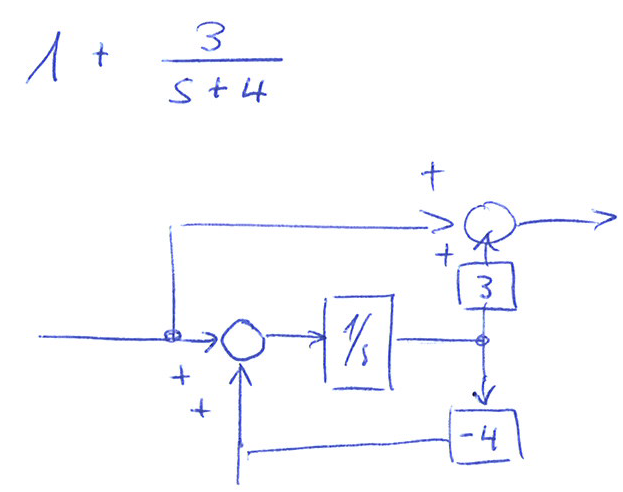
\includegraphics[width=5cm]{./images/implementierung2.png}
%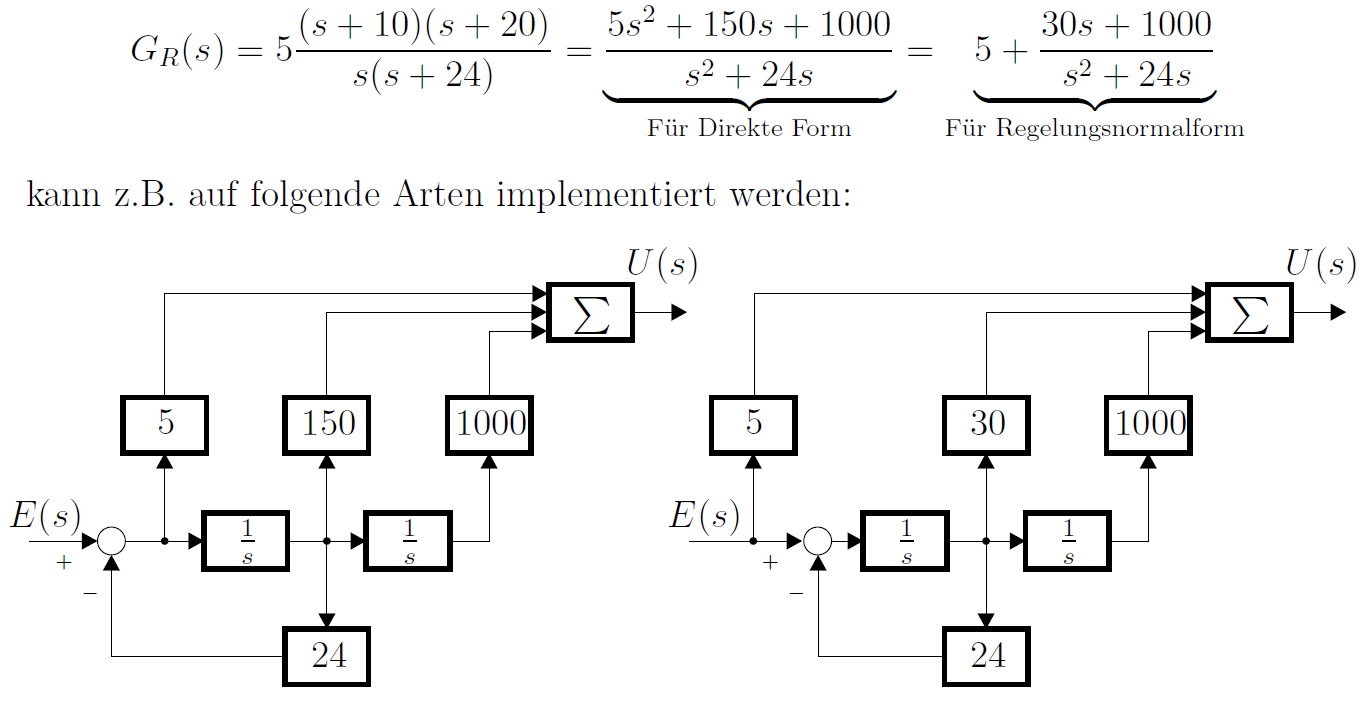
\includegraphics[width=10cm]{./images/implementierung.png}

\begin{center}
	\begin{longtable}{|p{0.25\textwidth}|c|}
	\hline
	\multicolumn{2}{|c|}{$G(S) = \frac{b_ms^m + b_{m-1}s^{m-1}+\dots + b_1s+b_0}{a_ns^n + a_{n-1}s^{n-1}+\dots + a_1s+a_0} \qquad (m\le n)$}\\
	\hline
	\textbf{Direkte Form/ Direkte Form II}
		& 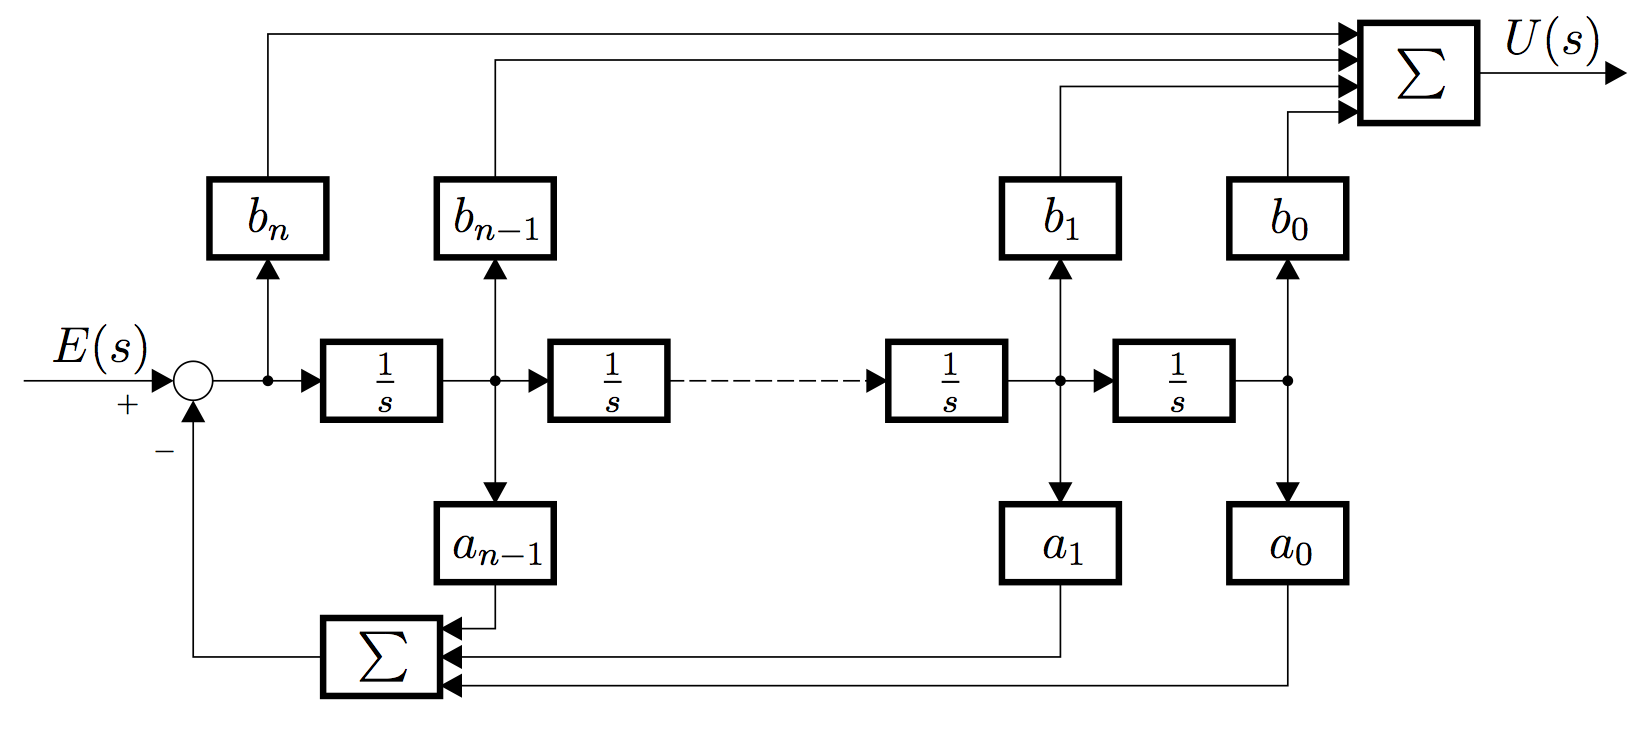
\includegraphics[width = 0.7\textwidth, height = 4.4cm]{./images/DirekteForm2}\\
	\hline
	\textbf{Transponierte direkte Form/ Direkte Form I}
		& 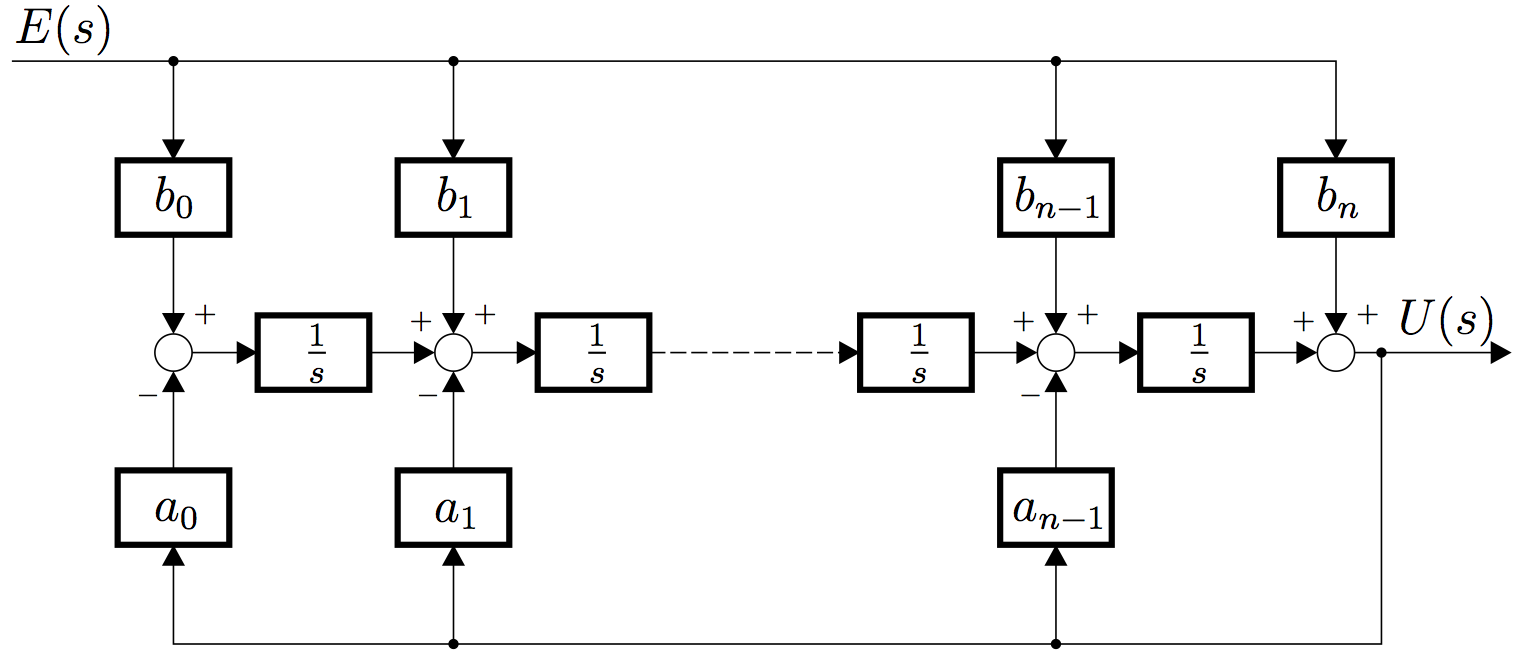
\includegraphics[width = 0.7\textwidth, height = 4.4cm]{./images/DirekteForm1}\\
	\hline
	\multicolumn{2}{|c|}{$G(S) = d + \frac{b_ms^m + b_{m-1}s^{m-1}+\dots + b_1s+b_0}{a_ns^n + a_{n-1}s^{n-1}+\dots + a_1s+a_0} \qquad (m < n)$}\\
	\hline
	\textbf{Regelungsnormalform}
		& 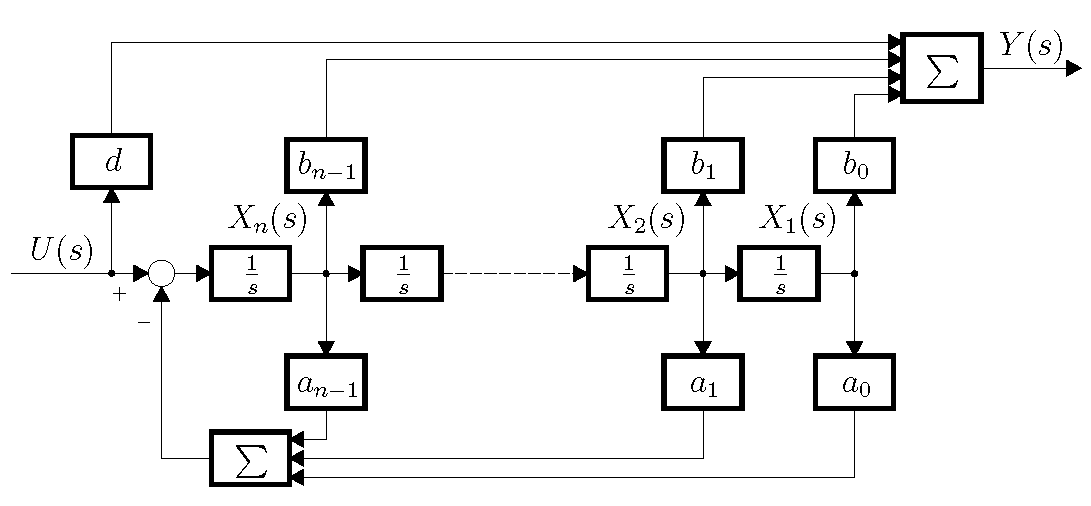
\includegraphics[width = 0.7\textwidth, height = 4.4cm]{./images/regelungsnormalform}\\
	\hline
	\end{longtable}
\end{center}

\section{Beispiele}
\section{Darstellung einiger gängiger WOK}
	\begin{figure}[h!]{13cm}
		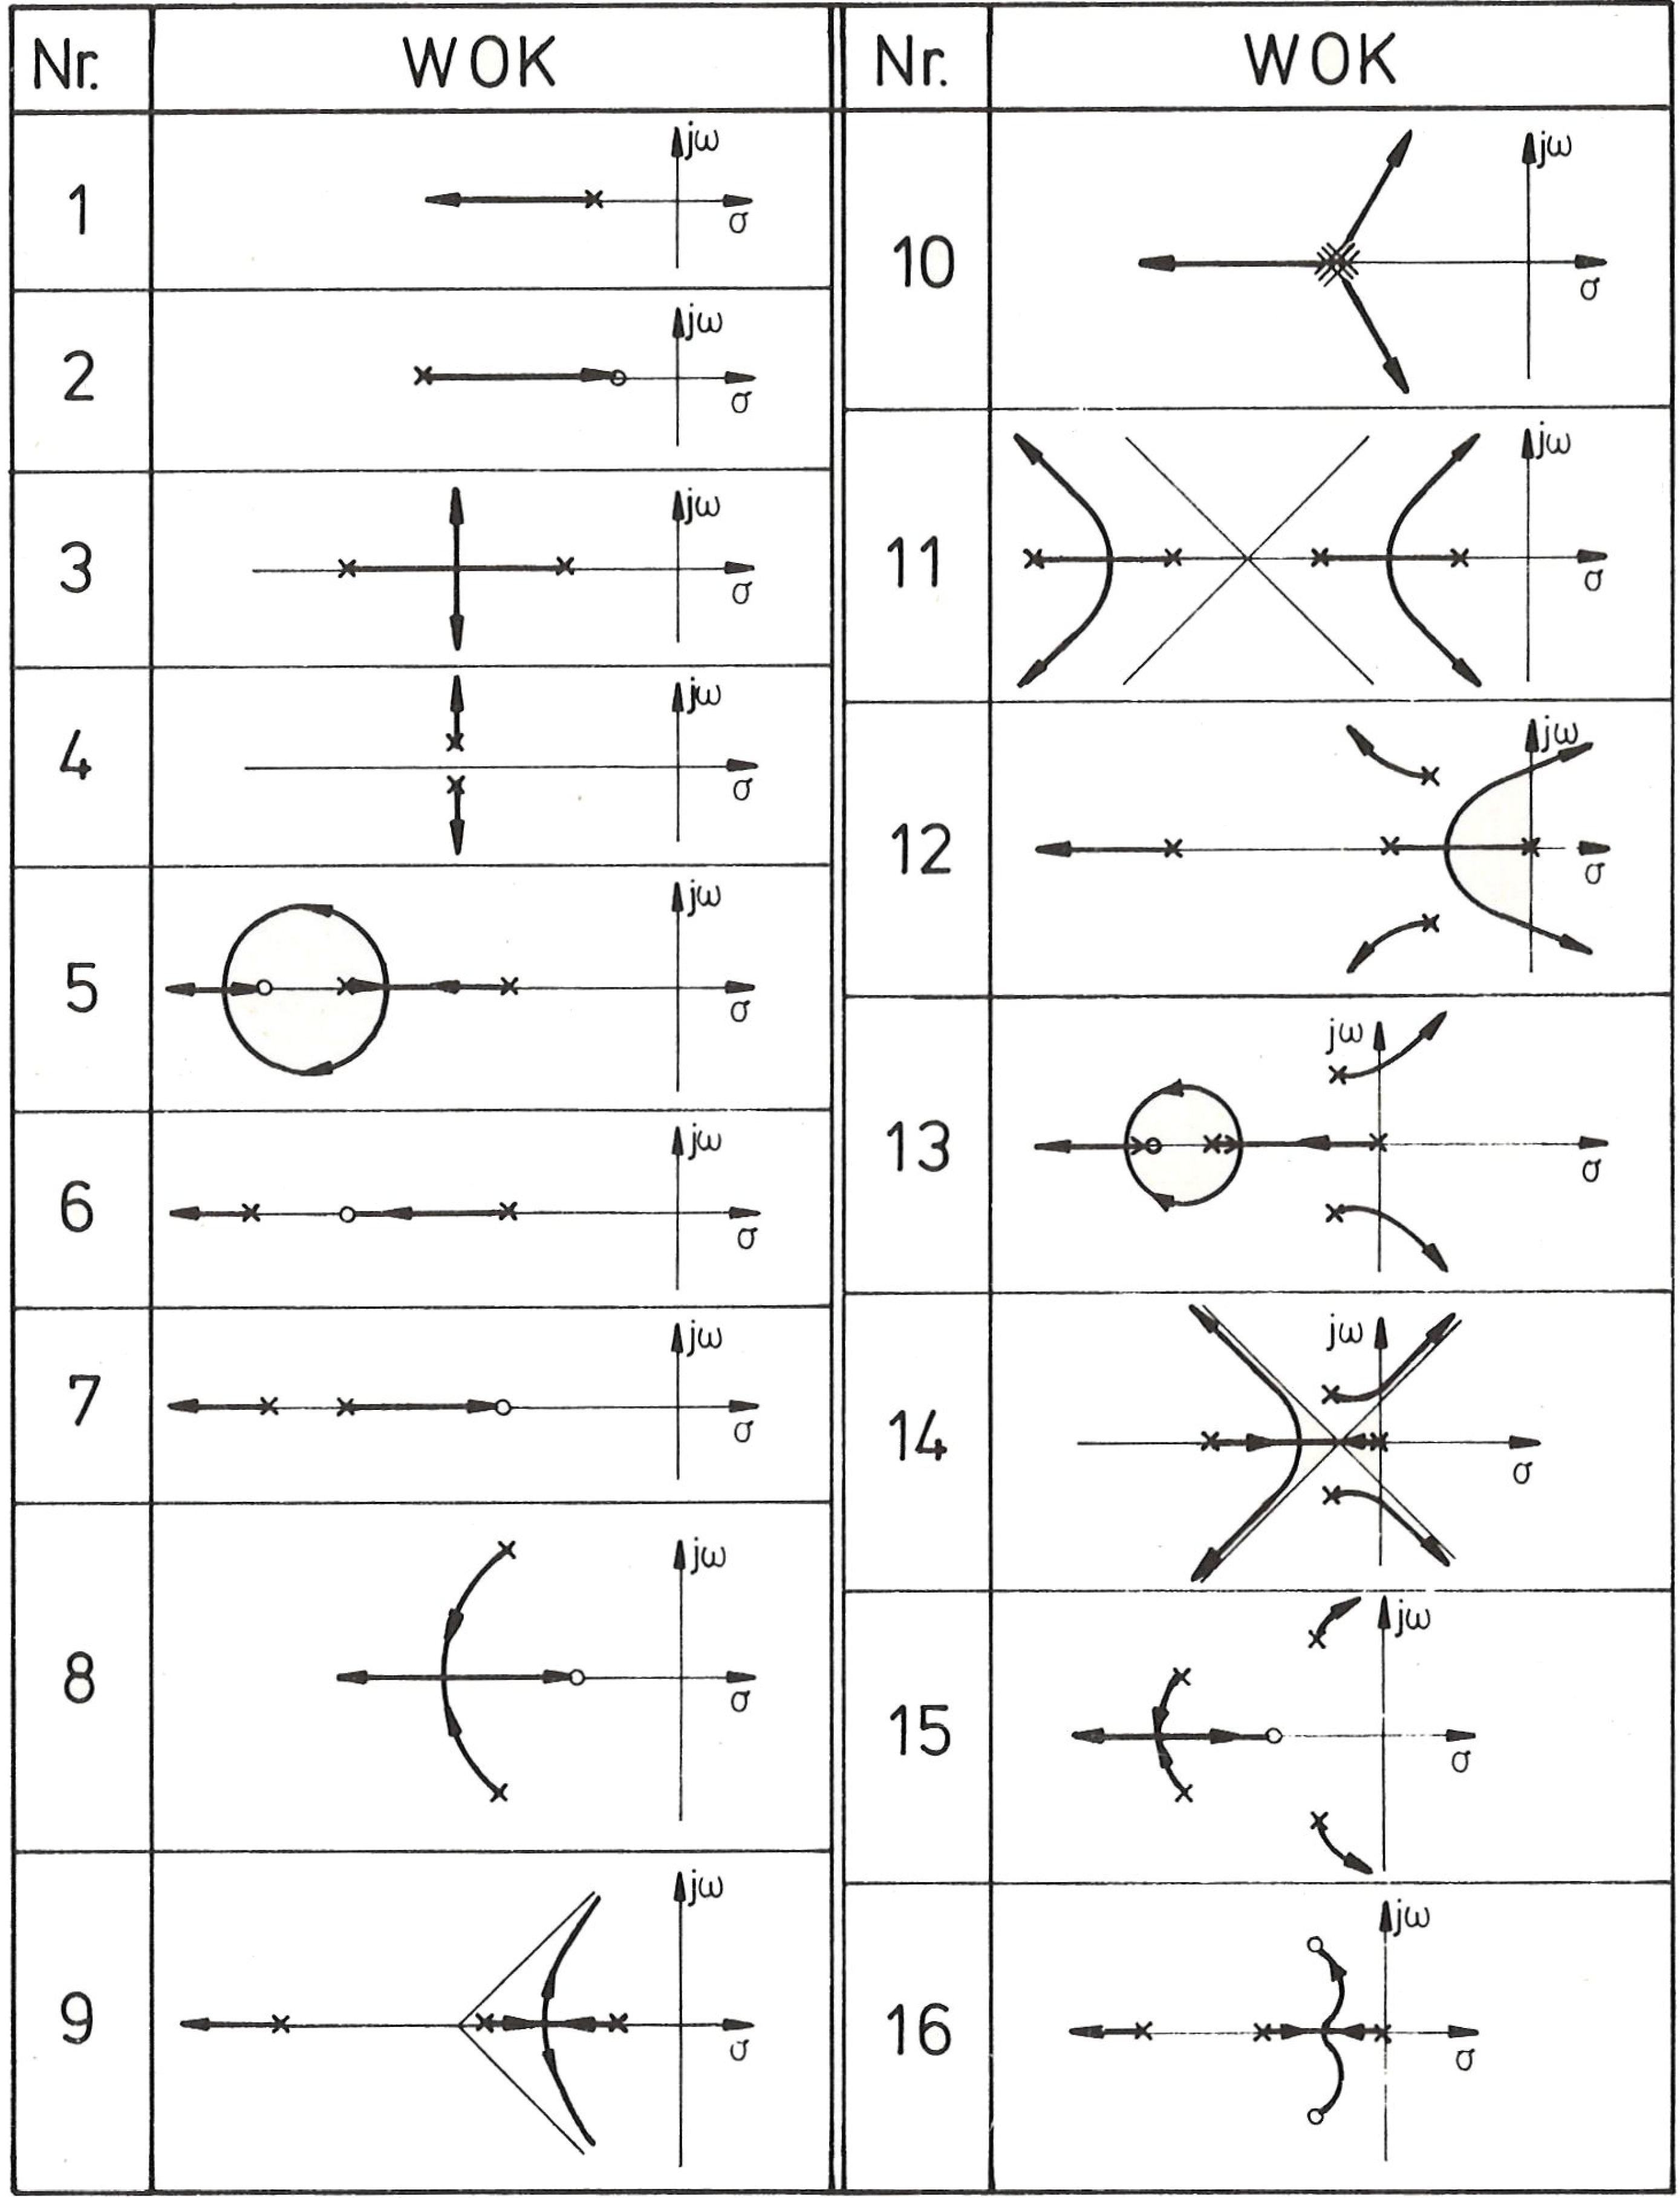
\includegraphics[width=11cm]{./images/BilderWOK.png}
		\caption{WOK zu einigen geläufigen Pol-/Nullstellenverteilungen, Quelle}
	\end{figure}
\end{document}
